% Copyright 2009 Ed Bueler
% based on example (directory) by Till Tantau:
%   /usr/share/doc/latex-beamer/examples/a-lecture/

\documentclass[10pt,hyperref={pdfpagelabels=true}]{beamer}

\usepackage{times}
\usepackage{hyperref}
\usepackage[T1]{fontenc}
\usepackage{verbatim}
\usepackage{empheq}
\usepackage{color}
%\usepackage{animate}
\usepackage{xmpmulti}  % more portable than animate
\usepackage{graphicx}


\newcommand{\ddt}[1]{\ensuremath{\frac{\partial #1}{\partial t}}}
\newcommand{\ddx}[1]{\ensuremath{\frac{\partial #1}{\partial x}}}
\newcommand{\ddy}[1]{\ensuremath{\frac{\partial #1}{\partial y}}}
\newcommand{\pp}[2]{\ensuremath{\frac{\partial #1}{\partial #2}}}
\renewcommand{\t}[1]{\texttt{#1}}
\newcommand{\Matlab}{\textsc{Matlab}\xspace}
\newcommand{\bq}{\mathbf{q}}
\newcommand{\bU}{\mathbf{U}}
\newcommand{\eps}{\epsilon}
\newcommand{\grad}{\nabla}
\newcommand{\Div}{\nabla\cdot}
\newcommand{\devstress}{\tau}

\newcommand{\mmess}[1]{\vspace{-0.1in}\begin{center}
\fbox{\url{#1.m}}
\end{center}}

\newcommand{\minput}[1]{\scriptsize\verbatiminput{tmp/#1.slim.m}
\tiny\mmess{#1}\normalsize}

\newcommand{\minputtiny}[1]{\tiny\verbatiminput{tmp/#1.slim.m}
\mmess{#1}\normalsize}



\title[Numerical modelling of ice sheets]{Numerical modelling of ice sheets, streams, and shelves}

\author[Bueler]{Ed Bueler}

\institute
{
%  Dept of Math \& Stat, and Geophysical Inst \\
  University of Alaska, Fairbanks \\
  \texttt{elbueler@alaska.edu}
}

\date{Lectures at McCarthy, Alaska, June 2016}



\begin{document}
\graphicspath{{../figures/}}


\begin{frame}
  \maketitle
\end{frame}

%\AtBeginSection[]{}

\AtBeginSection[]
{
  \begin{frame}<beamer>
    \frametitle{Outline}
    \tableofcontents[currentsection,hideallsubsections]
  \end{frame}
}



%\subsection{preamble}


\begin{frame}{slogans \& scope}

slogans: I will
  \begin{itemize}
  \item \alert{focus on approximating ice flow}
  \item \alert{provide numerical codes that actually work}
  \item \alert{always care about the continuum model}
  \end{itemize}
\medskip

scope: I will cover these
  \begin{itemize}
  \item models

    \begin{itemize}
    \item[$\circ$] shallow ice approximation (SIA) in 2D
    \item[$\circ$] shallow shelf approximation (SSA) in 1D
    \item[$\circ$] mass continuity \& surface kinematical equations
    \end{itemize}

  \item numerical ideas

    \begin{itemize}
    \item[$\circ$] finite difference schemes
    \item[$\circ$] solving algebraic systems from stress balances
    \item[$\circ$] verification
    \end{itemize}
  \end{itemize}
\end{frame}


\begin{comment}
\begin{frame}{outside of scope}

\large\emph{not} \normalsize covered here:\normalsize
\medskip

  \begin{itemize}
  \item Stokes and ``higher order'' flow equations
  \item thermomechanical coupling or polythermal ice
  \item subglacial hydrology/processes
  \item mass balance and snow/firn processes
  \item constitutive relations other than Glen isotropic
  \item grounding lines, calving fronts, ocean interaction
  \item paleo-climate and ``spin-up''
  \item earth deformation under ice sheet load
  \item other numerics: FEM, spectral, multigrid, parallel, \dots
  \item etc.
  \end{itemize}

\end{frame}
\end{comment}

\begin{frame}{notation} 

\begin{center}
  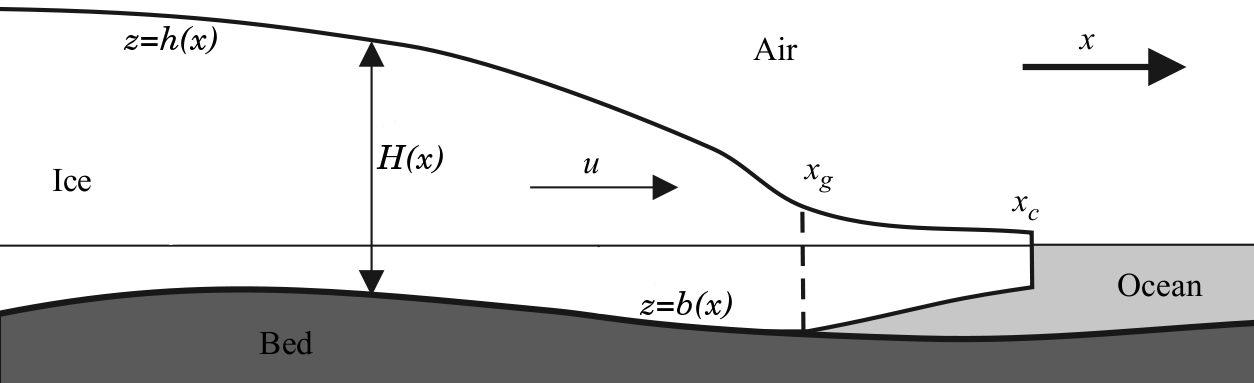
\includegraphics[width=0.9\textwidth]{flowline}

\tiny \emph{figure modified from} Schoof (2007)
\end{center}

\scriptsize
  \begin{itemize}
  \item coordinates $t,x,y,z$  (with $z$ vertical, positive upward)
  \item subscripts for partial derivatives $u_x = \partial u/\partial x$
  \item $H=$ ice thickness
  \item $h=$ ice surface elevation
  \item $b=$ bedrock surface elevation
  \item $T=$ temperature
  \item $\mathbf{u}=(u,v,w)=$ ice velocity
  \item $\rho=$ density of ice
  \item $\rho_w=$ density of ocean water
  \item $g=$ acceleration of gravity
  \item $n=3$ Glen flow law exponent $=3$
  \item $A=A(T)=$ ice softness in Glen law ($\mathbf{D}_{ij} = A(T) \tau^{n-1} \tau_{ij}$)
  \item \alert{please ask about notation!}
  \end{itemize}

\end{frame}


\begin{frame}{Matlab/Octave codes}

\begin{itemize}
\item lectures and notes are structured around 18 ice flow codes
\item several codes will appear in these lectures, but not all
\item each is $\sim$ 1/2 page of Matlab/Octave code
\item please give them a try!

  \begin{itemize}
  \item[$\circ$] \texttt{.zip} and \texttt{.tar.gz} forms available from memory stick
  \item[$\circ$] and online:

  \bigskip\bigskip\small
  \centerline{\fbox{\url{https://github.com/bueler/mccarthy}}}
  
  \end{itemize}
\end{itemize}
\end{frame}


\section[introduction]{introduction: a view from outside glaciology}

\subsection{ice flow equations}

\begin{frame}{ice in glaciers is treated a \emph{fluid}}

\begin{itemize}
\item what's a fluid?

\bigskip\bigskip
\item<2> at minimum, we describe fluids by
  \begin{itemize}
  \item[$\circ$] a \emph{density field}\quad $\rho(t,x,y,z)$
  \item[$\circ$] a vector \emph{velocity field}\quad $\mathbf{u}(t,x,y,z)$
  \end{itemize}
\end{itemize}
\end{frame}


\begin{frame}{ice in glaciers is a \emph{fluid} \quad 2}

\begin{itemize}
\item if the ice were
  \begin{itemize}
  \item[$\circ$] faster-moving than it actually is, and
  \item[$\circ$] linearly-viscous like liquid water
  \end{itemize}
  
  then it would be a ``typical'' fluid

\bigskip
\item for some typical fluids one uses the Navier-Stokes equations as the model:
\begin{align*}
\nabla \cdot \mathbf{u} &= 0 &&\text{\emph{incompressibility}} \\
\rho \left(\mathbf{u}_t + \mathbf{u}\cdot\nabla \mathbf{u}\right) &= -\nabla p + \nabla \cdot \tau_{ij} + \rho \mathbf{g} &&\text{\emph{force balance}} \\
2 \nu \mathbf{D}_{ij} &= \tau_{ij} &&\text{\emph{flow law}}
\end{align*}

\medskip
    \begin{itemize}
    \item[$\circ$] force balance equation is ``$m a = F$''    
    \end{itemize}
\end{itemize}
\end{frame}


\begin{frame}{\emph{hmmm} \dots \emph{does not sound like glaciology to me!}}

\begin{itemize}
\item \alert{yes}, numerical ice sheet flow modelling is ``computational fluid dynamics''
  \begin{itemize}
  \item[$\circ$] it's large-scale like atmosphere and ocean
  \item[$\circ$] \dots\, but it is a weird one
  \end{itemize}
\item consider what makes atmosphere/ocean flow exciting:
  \begin{itemize}
  \item[$\circ$] turbulence
  \item[$\circ$] convection
  \item[$\circ$] coriolis force
  \item[$\circ$] density/salinity stratification
  \item[$\circ$] chemistry (methane, ozone, \dots)
  \end{itemize}
\item none of the above list is relevant to ice flow
\item what could be interesting about the flow of slow, cold, stiff, laminar, inert old ice?
  \begin{itemize}
  \item[$\circ$] it's \emph{ice dynamics!}
  \end{itemize}
\end{itemize}
\end{frame}


\begin{frame}{ice is a slow, shear-thinning fluid}

\begin{itemize}
\item ice fluid is

\smallskip
  \begin{tabular}{lc}
  \emph{slow}\,: & $\rho \left(\mathbf{u}_t + \mathbf{u}\cdot\nabla \mathbf{u}\right) \approx 0$ \\
  \emph{non-Newtonian}\,: & viscosity $\nu$ is not constant
  \end{tabular}

\bigskip
\item ``slow'':
  $$\rho \left(\mathbf{u}_t + \mathbf{u}\cdot\nabla \mathbf{u}\right) \approx 0 \qquad \iff \qquad \begin{pmatrix} \text{forces of inertia} \\ \text{are neglected} \end{pmatrix}$$

\medskip
\item ice is non-Newtonian in a ``shear-thinning'' way
  \begin{itemize}
  \item[$\circ$] higher strain rates means lower viscosity
  \end{itemize}

\bigskip
\item so the standard ``full'' model is Glen-law ($n=3$) \alert{Stokes}:
\begin{align*}
\nabla \cdot \mathbf{u} &= 0 &&\text{\emph{incompressibility}} \\
0 &= - \nabla p + \nabla \cdot \tau_{ij} + \rho\, \mathbf{g} &&\text{\emph{force balance}} \\
\mathbf{D}_{ij} &= A \tau^2 \tau_{ij} &&\text{\emph{flow law}}
\end{align*}

\end{itemize}
\end{frame}


\begin{frame}{``slow'' means no memory of velocity (i.e.~momentum)}

\begin{itemize}
\item note \emph{no time derivatives} in Stokes model:
\scriptsize
\begin{align*}
\nabla \cdot \mathbf{u} &= 0 \\
0 &= - \nabla p + \nabla \cdot \tau_{ij} + \rho\, \mathbf{g} \\
\mathbf{D}_{ij} &= A \tau^2 \tau_{ij}
\end{align*}
\normalsize
\item thus a time-stepping ice sheet code
  \begin{itemize}
  \item[$\circ$] recomputes the full velocity field at every time step, and
  \item[$\circ$] does not require velocity from the previous time step\footnote{to paraphrase (?) Bob Dylan: to be a weather forecaster you've got to know which way the wind blows \dots but don't expect that from a glaciologist}
  \end{itemize}

\medskip
\item because there is no memory of previous velocity, velocity is a ``diagnostic'' output, not needed for (e.g.) restarting the model
\end{itemize}
\end{frame}


\subsection{slab-on-a-slope}

\begin{frame}{plane flow Stokes}

\begin{itemize}
\item recall the Stokes model:
\small
\begin{align*}
\nabla \cdot \mathbf{u} &= 0 &&\text{\emph{incompressibility}} \\
0 &= - \nabla p + \nabla \cdot \tau_{ij} + \rho\, \mathbf{g} &&\text{\emph{force balance}} \\
\mathbf{D}_{ij} &= A \tau^2 \tau_{ij} &&\text{\emph{flow law}}
\end{align*}
\normalsize

\bigskip
\item suppose we work in a $x,z$ plane, such as the centerline of a glacier, \emph{or} in a cross-flow plane

\item notation on next several slides:
  \begin{itemize}
  \item[$\circ$] $x,z$ as subscripts denote partial derivatives
  \item[$\circ$] $\tau_{13}$ is the ``vertical'' shear stress
  \item[$\circ$] $\tau_{11}$ and $\tau_{33}=-\tau_{11}$ are (deviatoric) longitudinal stresses 
  \end{itemize}
\end{itemize}
\end{frame}

\begin{frame}{plane flow Stokes  \quad 2}

\begin{itemize}
\item in the $x,z$ plane flow case the Stokes equations say
\begin{empheq}[]{align}
u_x + w_z &= 0 &&\text{\emph{incompressibility}}\notag \\
p_x &= \tau_{11,x} + \tau_{13,z} &&\text{\emph{stress balance} ($x$)} \notag \\
p_z &= \tau_{13,x} - \tau_{11,z} - \rho g &&\text{\emph{stress balance} ($z$)} \notag \\
u_x &= A \tau^2 \tau_{11} &&\text{\emph{flow law} (diagonal)}\notag \\
u_z + w _x &= 2 A \tau^2 \tau_{13} &&\text{\emph{flow law} (off-diagonal)} \notag
\end{empheq}
\item we have five equations in five unknowns ($u,w,p,\tau_{11},\tau_{13}$)
\item this is complicated enough \dots what about in a simplified situation?
\end{itemize}
\end{frame}


\begin{frame}{slab-on-a-slope}

\vspace{-0.05in}
\small

\begin{columns}

\begin{column}{0.5\textwidth}
\begin{itemize}
\item suppose: constant thickness, tilted bedrock
\item rotated coordinates:
  $$\mathbf{g} = g \sin\theta\, \hat x - g \cos \theta \,\hat z$$
\item so $p_x,p_z$ equations are now:
\begin{align}
p_x &= \tau_{11,x} + \tau_{13,z} + \rho g \sin\theta \notag \\
p_z &= \tau_{13,x} - \tau_{11,z} - \rho g \cos\theta \notag
\end{align}
\end{itemize}
\end{column}

\begin{column}{0.5\textwidth}
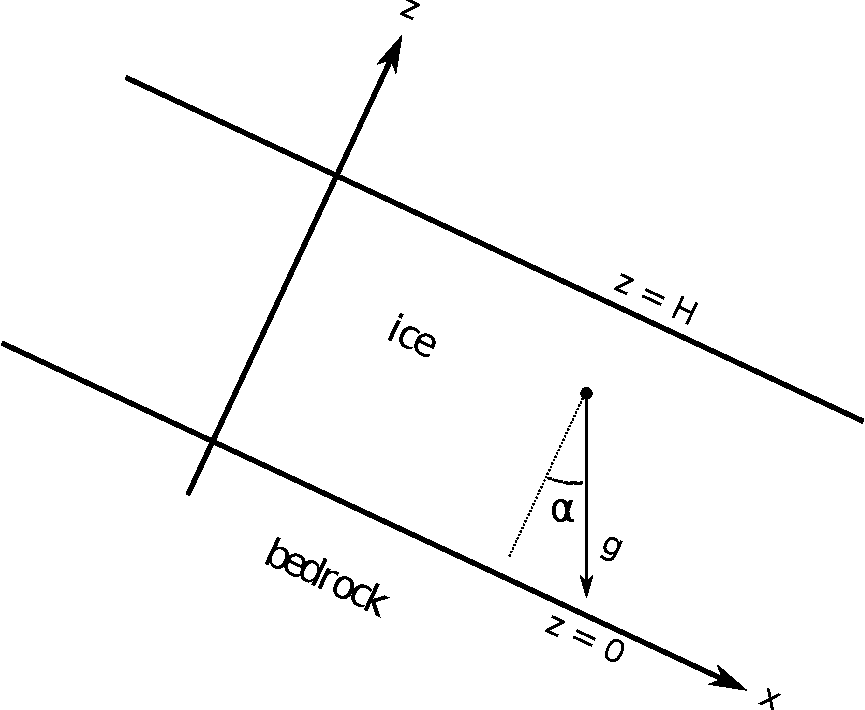
\includegraphics[width=1.0\textwidth]{slab}
\end{column}

\end{columns}

\begin{itemize}
\item for this \alert{slab-on-a-slope} there is \emph{no variation in} $x$
\item the equations simplify:
\small
\begin{empheq}[box=\fbox]{align}
w_z &= 0 &   0 &= \tau_{11} \notag \\
\tau_{13,z} &= - \rho g \sin\theta &   u_z &= 2 A \tau^2 \tau_{13} \notag \\
p_z &= - \rho g \cos\theta \notag
\end{empheq}
\normalsize
\end{itemize}
\end{frame}


\begin{frame}{slab-on-a-slope 2}

\begin{itemize}
\item add some boundary conditions:
	$$w(\text{base})=0, \qquad p(\text{surface})=0, \qquad u(\text{base})=u_0$$
\item by integrating vertically, get:
  $$w=0, \qquad p = \rho g \cos\theta (H-z), \qquad \tau_{13} = \rho g \sin\theta (H-z)$$
\item and from ``$u_z = 2 A \tau^2 \tau_{13}$'' get \alert{velocity formula}
\vspace{-0.05in}
\begin{align*}
u(z) &= u_0 + 2 A (\rho g \sin\theta)^3 \int_0^z (H-z')^3\,dz' \\
     &= u_0 + \frac{1}{2} A (\rho g \sin\theta)^3  \left(H^4 - (H-z)^4\right)
\end{align*}
\end{itemize}

\begin{center}
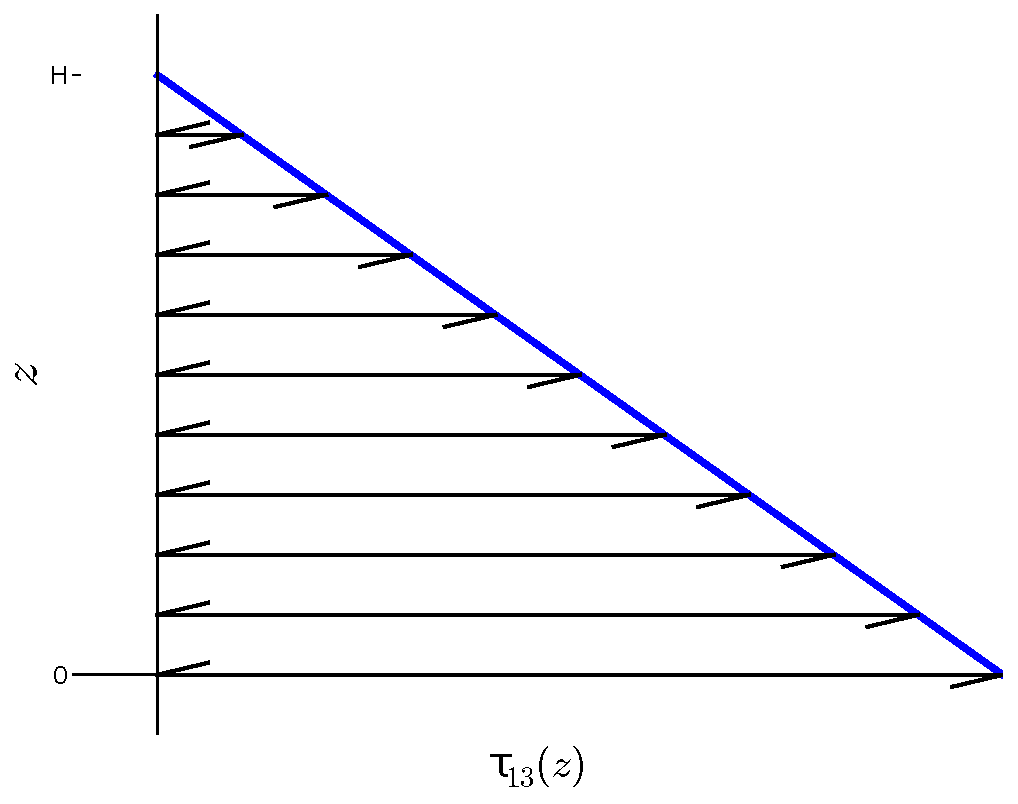
\includegraphics[width=0.4\textwidth]{slabshear}
\end{center}
\end{frame}


\begin{frame}{slab-on-a-slope 3}

\begin{columns}
\begin{column}{0.6\textwidth}
\begin{itemize}
\item do we believe these equations?
\item velocity formula on last slide gives figure below
\item compare to observations at right
\end{itemize}
\begin{center}
% NOT preserving aspect ratio
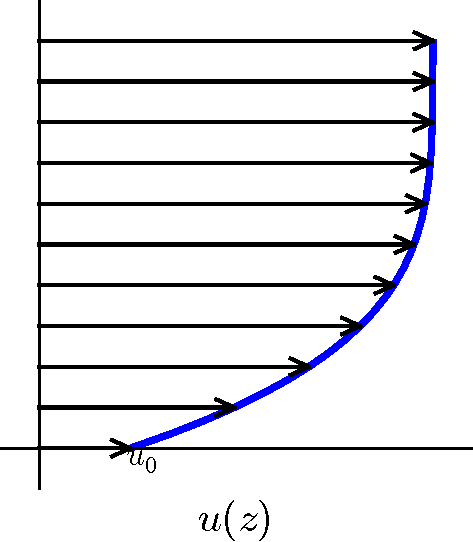
\includegraphics[width=0.6\textwidth,height=0.5\textheight]{slabvel}
\end{center}
\end{column}

\begin{column}{0.4\textwidth}
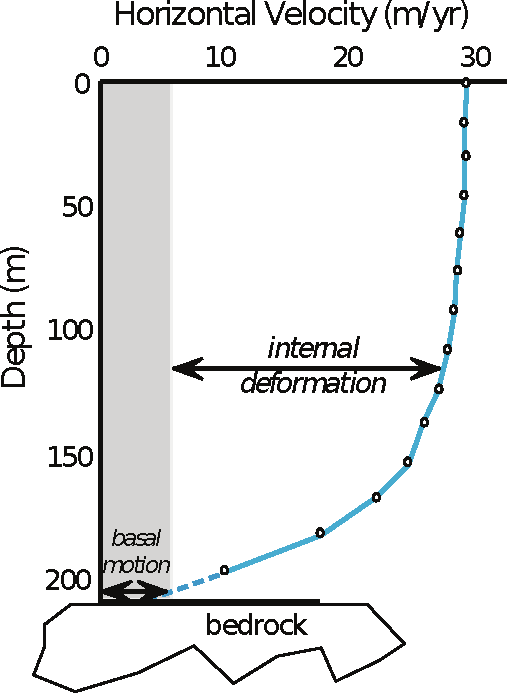
\includegraphics[width=1.0\textwidth]{athabasca-deform}

\medskip
\scriptsize
Velocity profile of the Athabasca Glacier, Canada, derived from inclinometry (Savage and Paterson, 1963)
\end{column}
\end{columns}
\end{frame}


\begin{frame}{mass conservation}

\begin{itemize}
\item \emph{Q}: having computed the velocity $u=u(t,x,z)$ \dots so what?
\item<2> \emph{A}: velocity moves the ice around \dots we want to predict where it goes 

\bigskip
\item<2> here we start to take \alert{a ``glacier-suitable'' view of mass conservation}
\item<2> suppose, instead of slab-on-a-slope, that our ice flow has variable thickness $H(t,x)$
\item<2> compute the vertical average of velocity:
	$$\bar u(t,x) = \frac{1}{H}\int_0^{H} u(t,x,z)\,dz$$
\end{itemize}
\end{frame}


\begin{frame}{mass conservation \quad 2}

\begin{columns}
\begin{column}{0.6\textwidth}
\small
\begin{itemize}
\item $M(x)$ is climatic(-basal) mass balance at $x$
\item consider change of area in the figure:
	$$\frac{dA}{dt} \stackrel{\ast}{=} \int_{x_1}^{x_2} M(x)\,dx + \bar u_1 H_1 - \bar u_2 H_2$$
\item assume width $dx=x_2-x_1$ is small so $A\approx dx\, H$
\item divide eqn $\ast$ by $dx$ and get
   $$H_t = M - \left(\bar u H\right)_x$$
\item this is a \emph{mass continuity equation}
\item area in 2D becomes volume in 3D
\end{itemize}
\end{column}
\begin{column}{0.4\textwidth}
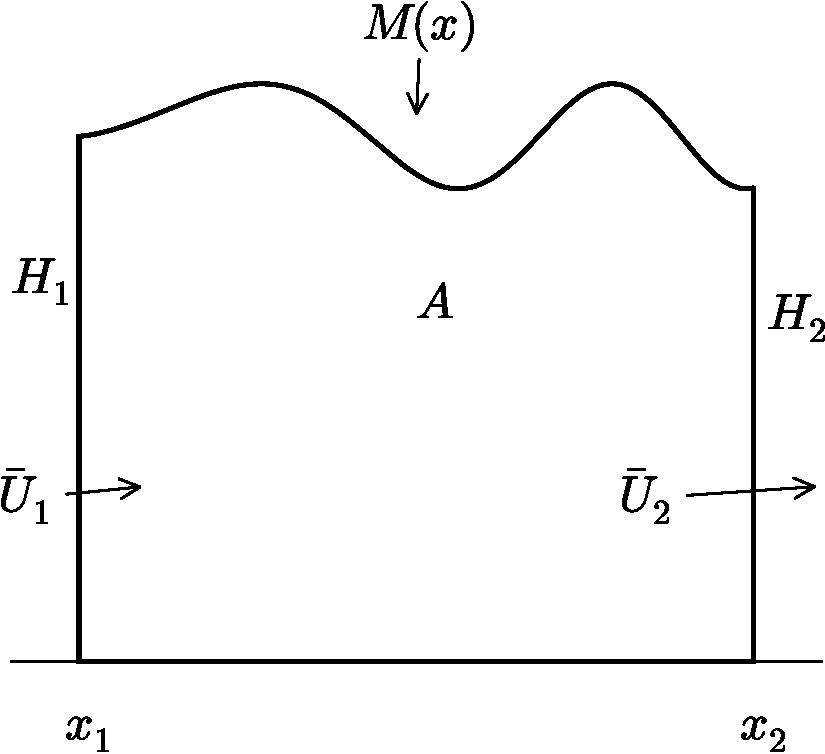
\includegraphics[width=1.0\textwidth]{slabmasscontfig}
\end{column}
\end{columns}

\end{frame}


\begin{frame}{combine equations so far}

\begin{itemize}
\item from slab-on-slope velocity formula in $u_0=0$ case,
\begin{align*}
\bar u H &= \int_0^H \frac{1}{2} A (\rho g \sin\theta)^3  \left(H^4 - (H-z)^4\right)\,dz \\
	&= \frac{2}{5} A (\rho g \sin\theta)^3 H^5
\end{align*}
\item note $\sin \theta \approx \tan\theta = - h_x$
\item combine with mass continuity $H_t = M - \left(\bar u H\right)_x$ to get:
  $$H_t = M + \left(\frac{2}{5} (\rho g)^5 A H^5 |h_x|^2 h_x\right)_x$$

\medskip
\item this is a rough explanation of ``shallow ice approximation'' (SIA) \dots next
\end{itemize}
\end{frame}




\section{shallow ice sheets}

\begin{frame}{slow, non-Newtonian, shallow, and sliding}

\begin{itemize}
\item ice sheets have four outstanding properties \emph{as fluids}:
  \begin{enumerate}
  \item slow
  \item non-Newtonian
  \item shallow (usually)
  \item contact slip (sometimes)
  \end{enumerate}
\end{itemize}
\end{frame}


\begin{frame}{regarding ``shallow''}

\begin{itemize}
\item below in \alert{red} is a no-vertical-exaggeration cross section of Greenland at $71^\circ$
\small
\item green and blue: standard vertically-exaggerated cross section
\item you can scale Stokes equation using smallness of $\eps = [H]/[L]$, where $[H]$ is a typical thickness of an ice sheet and $[L]$ is a typical horizontal dimension, \dots (Fowler, 1997)\nocite{Fowler}
\end{itemize}

\begin{center}
  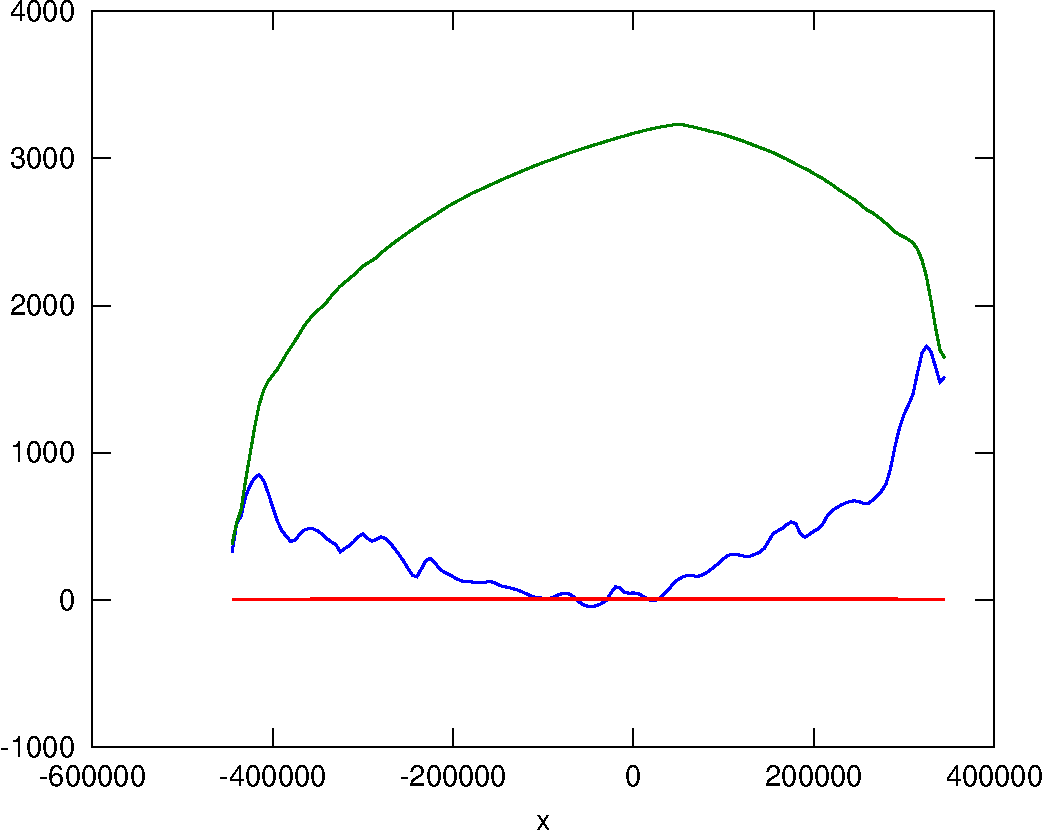
\includegraphics[width=0.6\textwidth]{green-transect}
\end{center}
\end{frame}


\subsection{shallow ice approx (SIA)}

\begin{frame}{flow model I: non-sliding, isothermal shallow ice approximation = (SIA)}

a model which applies to
\begin{itemize}
\item small depth-to-width ratio (``shallow'') grounded ice sheets
\item on not-too-rough bed topography,
\item whose flow is not dominated by sliding and/or liquid water at the base or margin
\end{itemize}

\begin{center}
  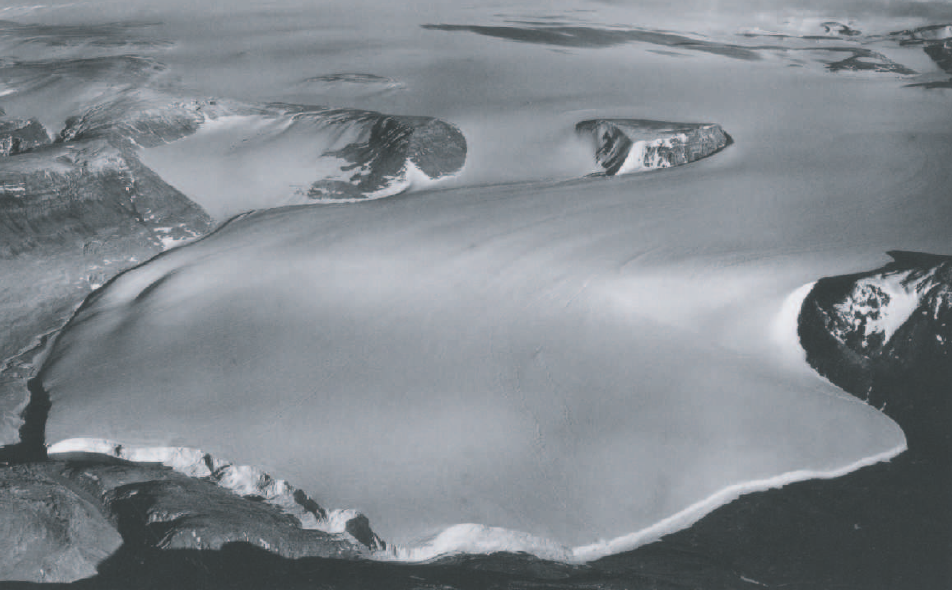
\includegraphics[width=0.65\textwidth]{polaris}

\tiny ``Polaris Glacier,'' northwest Greenland, photo 122, Post \& LaChapelle (2000)\nocite{PostLaChapelle}
\end{center}

\end{frame}


\begin{frame}{SIA model equations}

\begin{itemize}
\item \small though the best explanation of the SIA is to use shallowness to simplify the Stokes equations, here we take the simple slogan:\normalsize

\begin{center}
\emph{the SIA uses the formulas from slab-on-a-slope}
\end{center}
\item shear stress approximation:
	$$(\tau_{13},\tau_{23}) = - \rho g (h-z) \nabla h$$
\item let $\mathbf{u} = (u,v)$, the horizontal velocity
\item we further approximate
\begin{align*}
\mathbf{u}_z &= 2 A |(\tau_{13},\tau_{23})|^{n-1} (\tau_{13},\tau_{23}) \\
     &= - 2 A (\rho g)^n (h-z)^n |\nabla h|^{n-1} \nabla h
\end{align*}
\item by integrating vertically, in the non-sliding case,
    $$\mathbf{u} = - \frac{2 A (\rho g)^n}{n+1} \left[H^{n+1} - (h-z)^{n+1}\right] |\nabla h|^{n-1} \nabla h$$
\item but mass continuity remains, $H_t = M - \left(\overline{\mathbf{u}} H\right)_x$
\end{itemize}
\end{frame}


\begin{frame}{SIA thickness equation}

\begin{itemize}
\item from last slide, we get the non-sliding, isothermal shallow ice approximation for how thickness changes:
\begin{empheq}[box=\fbox]{equation}
H_t = M + \Div \left(\Gamma H^{n+2} |\grad h|^{n-1} \grad h \right) \label{sia}
\end{empheq}

\vspace{-2mm}
  \begin{itemize}
  \item[$\circ$] where $H$ is ice thickness, $h$ is ice surface elevation, $b$ is bed elevation ($h=H+b$)
  \item[$\circ$] $M$ combines surface and basal mass (im)balance:

     accumulation if $M>0$, ablation if $M<0$
  \item[$\circ$] $n$ is the exponent in the Glen flow law
  \item[$\circ$] $\Gamma = 2 A (\rho g)^n / (n+2)$ is a positive constant
  \end{itemize}
\item numerically solve (1) and you've got a usable model for \dots \emph{the Barnes ice cap} (Mahaffy, 1976)\nocite{Mahaffy}
\end{itemize}
\medskip

\begin{columns}
\begin{column}{0.7\textwidth}
\small
\noindent good questions:
\begin{enumerate}
\item where does equation (1) come from?
\item how to solve it numerically?
\item how to \emph{think} about it?
\end{enumerate}  
\end{column}
\begin{column}{0.3\textwidth}
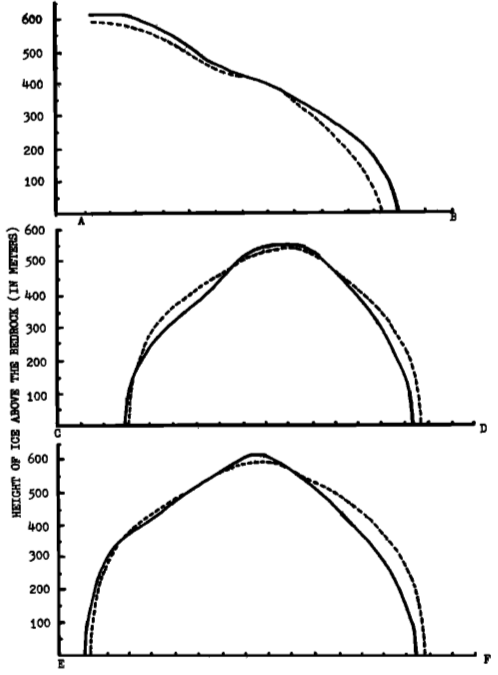
\includegraphics[width=0.8\textwidth]{mahaffy-profiles}
\end{column}
\end{columns}
\end{frame}


\subsection{analogy w heat equation}

\begin{frame}{heat equation}
\label{slide:heatcompare}

\small
\begin{columns}
\begin{column}{0.6\textwidth}
\begin{itemize}
\item for understanding SIA, recall heat equation
\item recall Newton's law of cooling
	$$\frac{dT}{dt} = -K (T-T_{\text{ambient}})$$
where $T$ is object temperature and $K$ relates to material and geometry of object (e.g.~cup of coffee)
\item Newton's law for segments of a rod:
\begin{align*}
\frac{dT_j}{dt} &= -K \left(T_j - \frac{1}{2} (T_{j-1} + T_{j+1}) \right) \\
	&= \frac{K}{2} \left(T_{j-1} - 2 T_j + T_{j+1}\right) 
\end{align*}
\item this has limit as segments shrink:
	$$T_t = D T_{xx}$$
\item compare: finite difference approximations to derivatives
\end{itemize}
\end{column}

\begin{column}{0.4\textwidth}
\hfill

\includegraphics[width=0.5\textwidth]{coffee}
\vspace{1.0in}
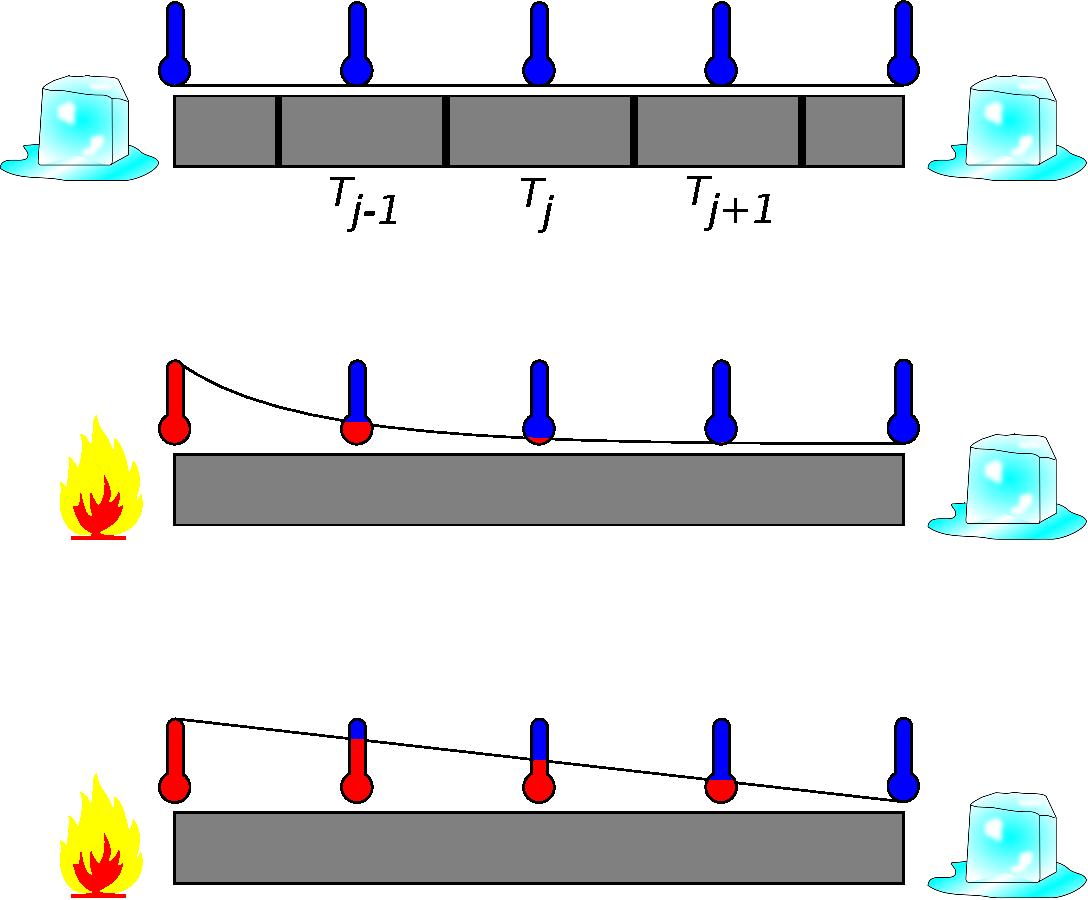
\includegraphics[width=1.0\textwidth]{heatconduction}
\end{column}
\end{columns}
\end{frame}

\begin{frame}{analogy: SIA versus 2D heat equation}

\begin{itemize}
\item side-by-side comparison:
\begin{center}
\begin{tabular}{cc}
\scriptsize SIA:\, $H(t,x,y)$ is ice thickness & \scriptsize heat: $T(t,x,y)$ is temperature \normalsize \\
	\boxed{H_t = M + \Div \left({\color{red}\Gamma H^{n+2} |\grad h|^{n-1}}\, \grad h \right)}  &  \boxed{T_t = F + \Div (D\, \grad T)}
\end{tabular}
\end{center}

\medskip
\item we identify the diffusivity in the SIA:
	$$D = {\color{red}\Gamma H^{n+2} |\grad h|^{n-1}}$$
\item \emph{non-sliding shallow ice flow \alert{diffuses} the ice sheet}
\item some issues with this analogy:
  \begin{itemize}
  \item[$\circ$]  $D$ depends on solution $H(t,x,y)$
  \item[$\circ$]  $D\to 0$ at margin, where $H\to 0$
  \item[$\circ$]  $D\to 0$ at divides/domes, where $|\grad h|\to 0$
  \end{itemize}
\end{itemize}
\end{frame}


\subsection{finite difference numerics}

\begin{frame}{numerics for heat equation: basic ideas of finite differences}

\begin{itemize}
\item numerical schemes for heat equation are good start for SIA
\item for differentiable $f(x)$ and any $h$, \emph{Taylor's theorem} says
	$$f(x+h) = f(x) + f'(x) h + \frac{1}{2} f''(x) h^2 + \frac{1}{3!} f'''(x) h^3 + \dots$$
\normalsize
\item you can replace ``$h$'' by multiples of $\Delta x$, e.g.:
\small
\begin{align*}
f(x-\Delta x) &= f(x) - f'(x) \Delta x + \frac{1}{2} f''(x) \Delta x^2 - \frac{1}{3!} f'''(x) \Delta x^3 + \dots \\
f(x+2\Delta x) &= f(x) + 2 f'(x) \Delta x + 2 f''(x) \Delta x^2 + \frac{4}{3} f'''(x) \Delta x^3 + \dots
\end{align*}
\normalsize
\item \emph{combine expressions like these to give approximations of derivatives, from values on a grid}
\end{itemize}
\end{frame}


\begin{frame}{finite differences for partial derivatives}

\begin{itemize}
\item we want partial derivative expressions, for example with any function $u=u(t,x)$:
\small
\begin{align*}
u_t(t,x) &= \frac{u(t+\Delta t,x) - u(t,x)}{\Delta t} + O(\Delta t), \\
u_t(t,x) &= \frac{u(t+\Delta t,x) - u(t-\Delta t,x)}{2\Delta t} + O(\Delta t^2), \\
u_x(t,x) &= \frac{u(t,x+\Delta x) - u(t,x-\Delta x)}{2\Delta x} + O(\Delta x^2), \\
u_{xx}(t,x) &= \frac{u(t,x+\Delta x) - 2 u(t,x) + u(t,x-\Delta x)}{\Delta x^2} + O(\Delta x^2)
\end{align*}
\normalsize
and so on
\item sometimes we want a derivative in-between grid points:
\small
	$$u_x(t,x+(\Delta x/2)) = \frac{u(t,x+\Delta x) - u(t,x)}{\Delta x} + O(\Delta x^2)$$
\normalsize
\item ``$+O(h^2)$'' is better than ``$+O(h)$'' if $h$ is a small number
\end{itemize}
\end{frame}


\begin{frame}{explicit scheme for heat equation}
\label{slide:explicit}

\begin{itemize}
\item consider 1D heat equation $T_t = D T_{xx}$
\item an \emph{explicit} scheme comes from:
\small
	$$\frac{T(t+\Delta t,x) - T(t,x)}{\Delta t} \approx D\,\frac{T(t,x+\Delta x) - 2 T(t,x) + T(t,x-\Delta x)}{\Delta x^2}$$
\normalsize
\item the difference between the equation $T_t = D T_{xx}$ and the scheme is $O(\Delta t,\Delta x^2)$ (Morton and Mayers, 2005)\nocite{MortonMayers}
\item notation: $(t_n,x_j)$ is a point in the time-space grid
\item notation: $T_j^n \approx T(t_n,x_j)$
\item let $\nu = D \Delta t / (\Delta x)^2$, so scheme is
\small
	$$T_j^{n+1} = \nu T_{j+1}^n + (1 - 2 \nu) T_j^n + \nu T_{j-1}^n$$
\normalsize
\end{itemize}
\begin{columns}
\begin{column}{0.55\textwidth}
\begin{itemize}
\item scheme has stencil at right \large $\to$ \normalsize
\end{itemize}
\end{column}
\begin{column}{0.45\textwidth}
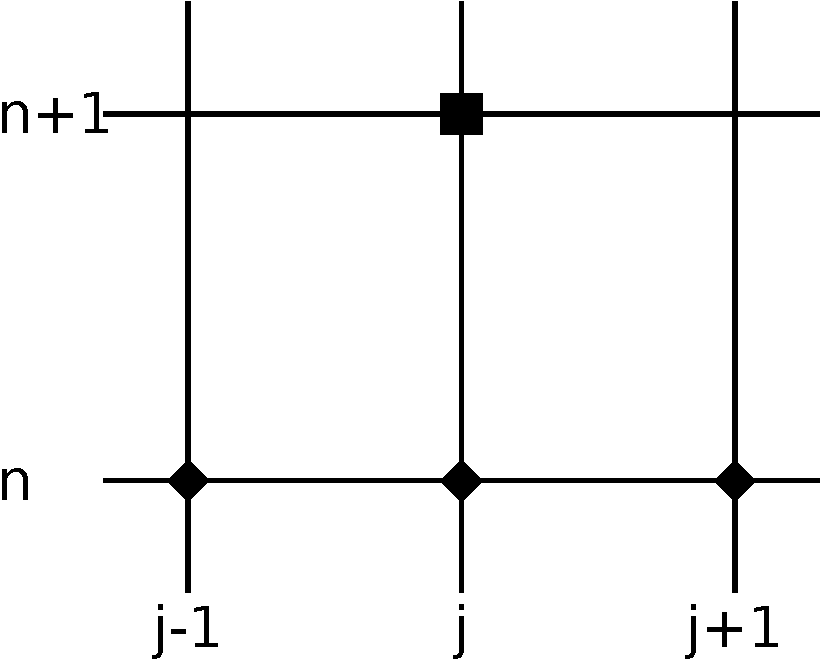
\includegraphics[width=0.7\textwidth]{expstencil}
\end{column}
\end{columns}
\end{frame}


\begin{frame}{explicit scheme in two space dimensions}

\begin{itemize}
\item recall heat equation in 2D: $T_t = D(T_{xx} + T_{yy})$
\item in two spatial variables we write $T_{jk}^n \approx T(t_n,x_j,y_k)$
\item so the 2D explicit scheme is
\small
	$$\frac{T_{jk}^{n+1} - T_{jk}^n}{\Delta t} = D\,\left(\frac{T_{j+1,k}^n - 2 T_{jk}^n + T_{j-1,k}^n}{\Delta x^2} + \frac{T_{j,k+1}^n - 2 T_{jk}^n + T_{j,k-1}^n}{\Delta y^2}\right)$$
\end{itemize}

\bigskip
\begin{center}
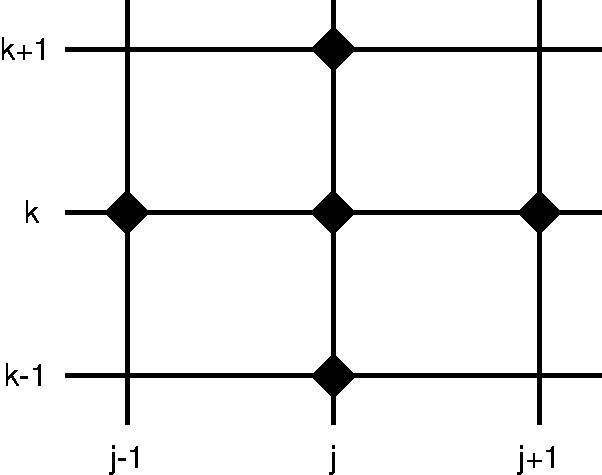
\includegraphics[width=0.45\textwidth]{exp2dstencil}
\end{center}
\end{frame}


\begin{frame}{implementation}
\label{slide:heatmatlab}

\minput{heat}

\small
\begin{itemize}
\item solves $T_t = D(T_{xx} + T_{yy})$ on square $-1 < x < 1$, $-1 < y < 1$
\item example uses initial condition $T_0(x,y) = e^{-30 r^2}$
\item code uses ``colon notation'' to remove loops (over space)
\item \texttt{>>  heat(1.0,30,30,0.001,20)}

approximates $T$ on $30\times 30$ spatial grid, with $D=1$ and $N=20$ steps of $\Delta t = 0.001$
\end{itemize}
\end{frame}


\begin{frame}{the look of success}

\begin{itemize}
\item solving $T_t = D(T_{xx} + T_{yy})$ on $30\times 30$ grid
\end{itemize}

\bigskip\bigskip
\begin{columns}
\begin{column}{0.5\textwidth}
initial condition $T(0,x,y)$

\bigskip
\begin{center}
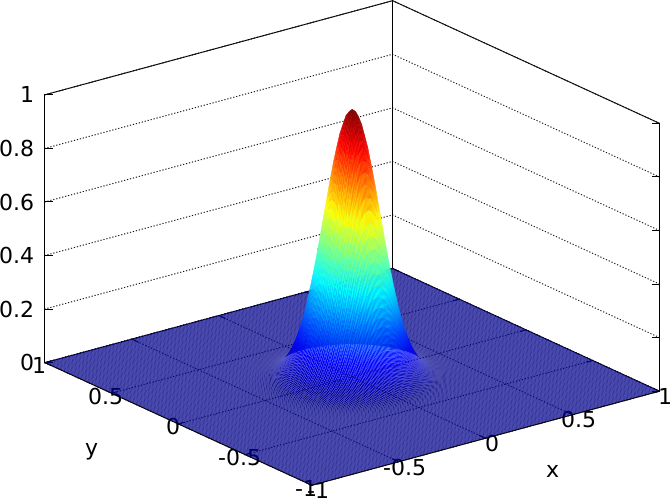
\includegraphics[width=1.0\textwidth]{initialheat}
\end{center}
\end{column}
\begin{column}{0.5\textwidth}
approximate solution $T(t,x,y)$ at $t=0.02$ with $\Delta t=0.001$ 

\bigskip
\begin{center}
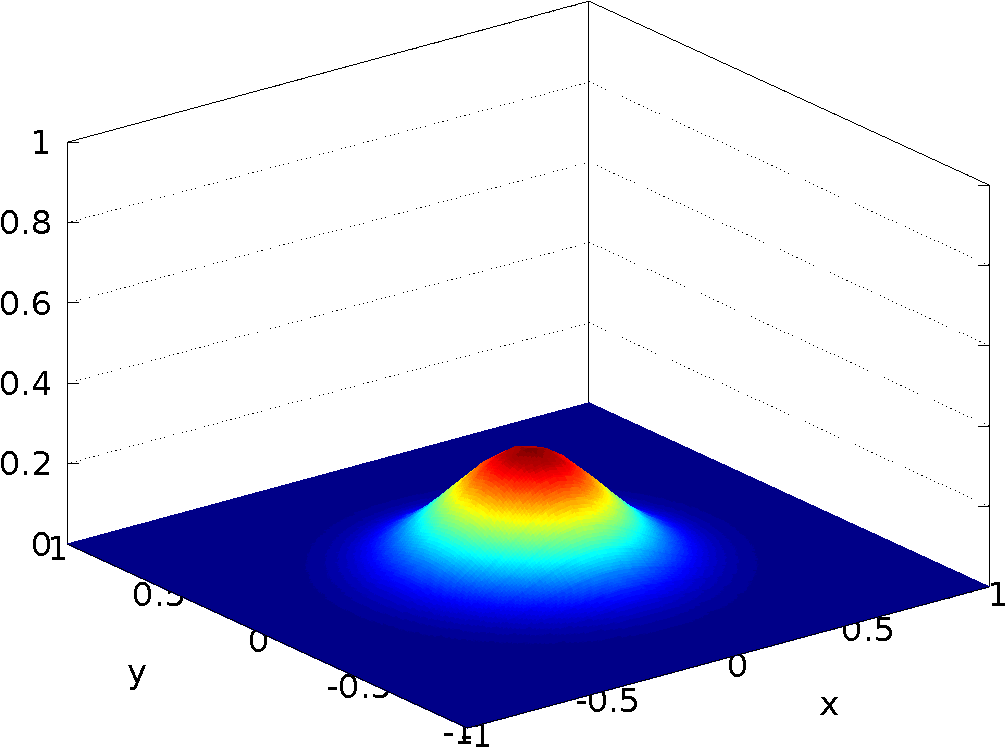
\includegraphics[width=1.0\textwidth]{finalheat}
\end{center}
\end{column}
\end{columns}
\end{frame}


\begin{frame}{the look of instability}

\begin{itemize}
\item both figures are from solving $T_t = D(T_{xx} + T_{yy})$ on the same space grid, but with slightly different time steps
\end{itemize}

\bigskip\bigskip
\begin{columns}
\begin{column}{0.5\textwidth}
\begin{center}
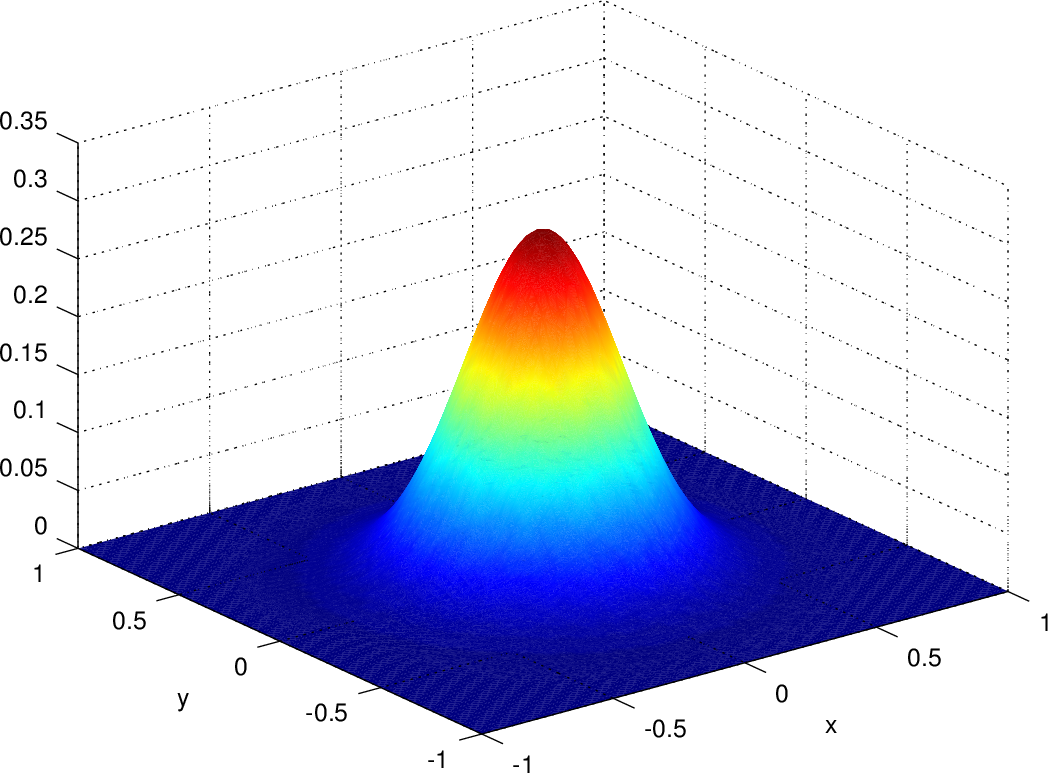
\includegraphics[width=1.0\textwidth]{stability}

%$D=1,\Delta t = 0.00064286,\Delta x = \Delta y = 0.04$ so
\uncover<2->{$$\frac{D\Delta t}{\Delta x^2}= 0.402$$}
\end{center}
\end{column}
\begin{column}{0.5\textwidth}
\begin{center}
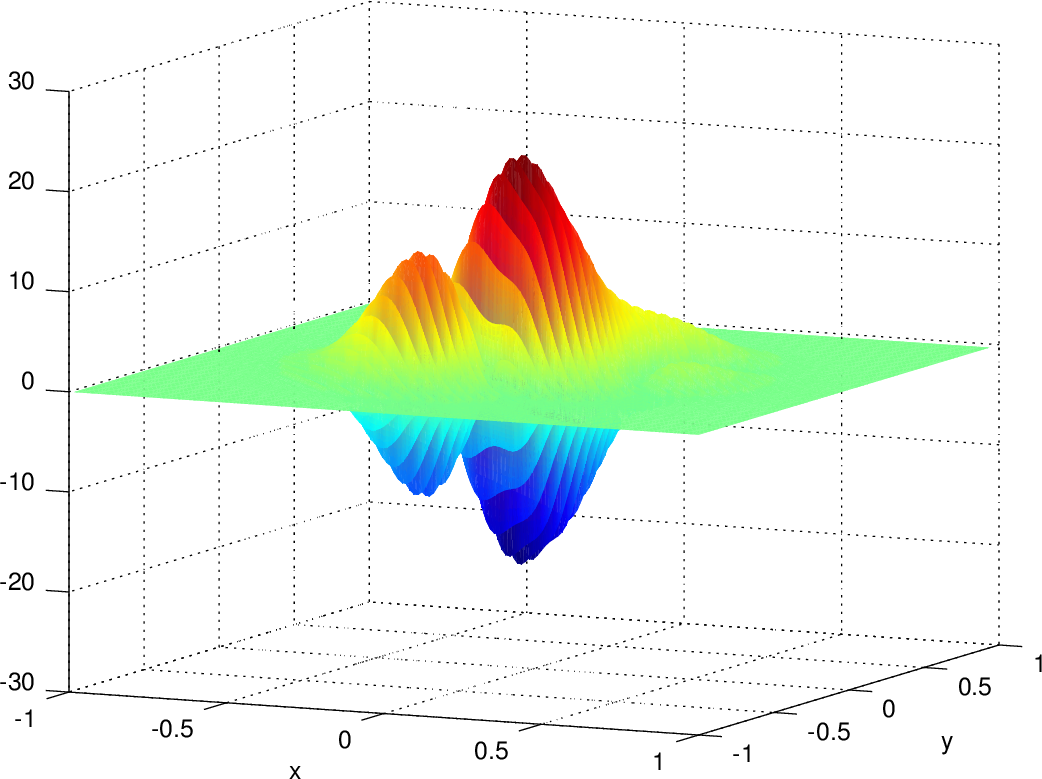
\includegraphics[width=1.0\textwidth]{instability}

%$D=1,\Delta t = 0.001,\Delta x = \Delta y = 0.04$ so
\uncover<2->{$$\frac{D\Delta t}{\Delta x^2}= 0.625$$}
\end{center}
\end{column}
\end{columns}
\end{frame}


\begin{frame}{avoid the instability}
\label{slide:maxprinc}

\begin{itemize}
\item recall 1D explicit scheme had the form 
	$$T_j^{n+1} = \nu T_{j+1}^n + (1 - 2 \nu) T_j^n + \nu T_{j-1}^n$$
\item thus the new value $u_j^{n+1}$ is an \emph{average} of the old values, \emph{if the middle coefficient is positive}:
	$$1 - 2 \nu \ge 0 \quad \iff \quad  \frac{D\Delta t}{\Delta x^2} \le \frac{1}{2} \quad \iff \quad \Delta t \le \frac{\Delta x^2}{2 D}$$
\item averaging is always stable because averaged wiggles are always smaller than the original wiggles
\item \dots so this condition is a sufficient \emph{stability criterion}
\item so:

\begin{center}
\emph{the result was unstable because the time step was too big}
\end{center}
\end{itemize}
\end{frame}


\begin{frame}{\textsl{adaptive} implementation: guaranteed stability}

\minput{heatadapt}

\begin{itemize}
\item same as \texttt{heat.m} except

\begin{center}
\emph{choose time step from stability criterion}
\end{center}
\end{itemize}\end{frame}


\begin{frame}{alternative instability fix: implicitness}

\begin{itemize}
\item \alert{implicit} methods can be stable for \emph{any} positive time step $\Delta t$
\end{itemize}

\begin{columns}
\begin{column}{0.7\textwidth}
\small
\begin{itemize}
\item an implicit scheme is \emph{Crank-Nicolson} $\longrightarrow$
\item Crank-Nicolson has smaller error too: $O(\Delta t^2,\Delta x^2)$
\end{itemize}
\normalsize
\end{column}
\begin{column}{0.3\textwidth}
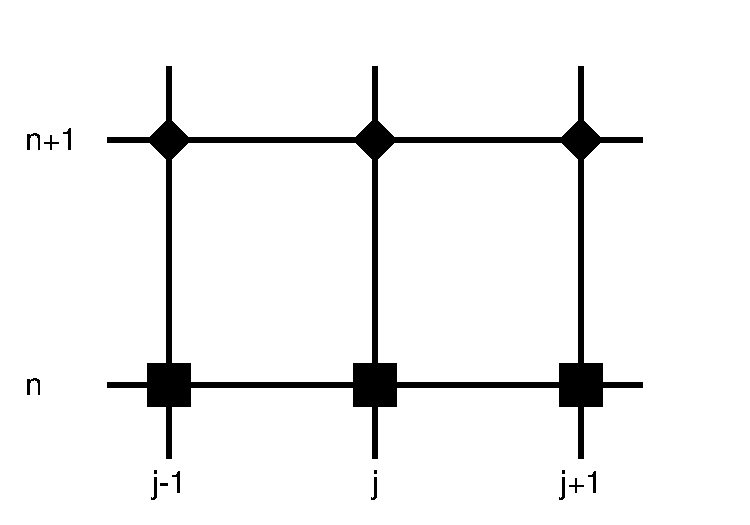
\includegraphics[width=1.2\textwidth]{cnstencil}
\end{column}
\end{columns}

\begin{itemize}
\item \emph{but} you have to solve linear (or nonlinear) systems of equations to take each time step
\medskip

\item \scriptsize Donald Knuth has advice for ice sheet modelers: \begin{quote}
\emph{We should forget about small efficiencies \dots: premature optimization is the root of all evil}.
\end{quote}
\end{itemize}
\end{frame}


\begin{frame}{variable diffusivity and time steps}

\begin{itemize}
  \item recall the analogy: \qquad (SIA) $\leftrightarrow$ (heat eqn)
  \item the SIA has a diffusivity which varies in space, so consider a more general heat equation:
  		$$T_t = F + \Div \left(D(x,y) \grad T\right)$$
  \item the explicit method is conditionally stable with the same time step restriction if we evaluate diffusivity $D(x,y)$ at \alert{staggered} grid points:
  \scriptsize
\begin{align*}
\Div \left(D(x,y) \grad u\right) &\approx \frac{D_{j+1/2,k}(T_{j+1,k} - T_{j,k}) - D_{j-1/2,k}(T_{j,k} - T_{j-1,k})}{\Delta x^2} \\
	&\qquad + \frac{D_{j,k+1/2}(T_{j,k+1} - T_{j,k}) - D_{j,k-1/2}(T_{j,k} - T_{j,k-1})}{\Delta y^2}
\end{align*}
\end{itemize}

\vspace{-0.15in}
\small
\begin{columns}
\begin{column}{0.55\textwidth}
in stencil at right:
\begin{itemize}
\item[] diamonds: $T$
\item[] triangles: $D$
\end{itemize}
\end{column}
\begin{column}{0.45\textwidth}
\begin{center}
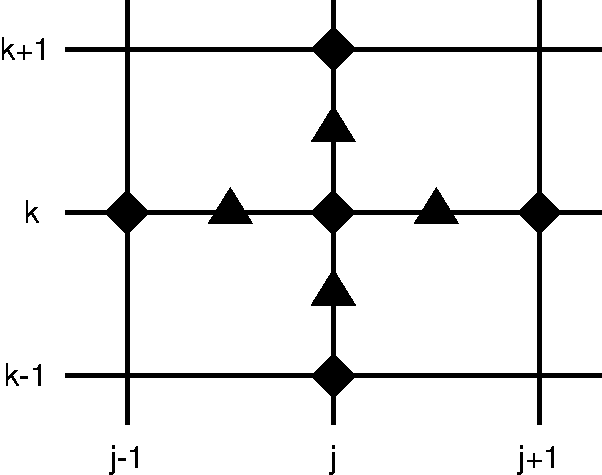
\includegraphics[width=1.0\textwidth]{diffstencil}
\end{center}
\end{column}
\end{columns}
\end{frame}


\begin{frame}
  \frametitle{general diffusion equation code}

\minputtiny{diffusion}

\small
\begin{itemize}
\item solves abstract diffusion equation $T_t = \Div \left(D(x,y)\, \grad T\right)$
\item user supplies diffusivity on staggered grid
\end{itemize}
\end{frame}


\subsection{solutions}

\begin{frame}{verification of numerical ice flow codes}
\begin{itemize}
\item how do we make sure an \emph{implemented} numerical scheme is correct?
  \begin{itemize}
  \item[$\circ$] \emph{technique} 1: don't make any mistakes
  \item[$\circ$] \emph{technique} 2: compare your model with others, and hope that the outliers are the ones with errors
  \item[$\circ$] \emph{technique} 3: build-in a comparison to an exact solution, and actually measure the numerical error $=$ \alert{verification}
  \end{itemize}

\medskip
\item where to get exact solutions for ice flow models?
  \begin{itemize}
  \item[$\circ$] textbook: Greve and Blatter (2009)\nocite{GreveBlatter2009}
  \item[$\circ$] similarity solutions to SIA (Halfar 1983\nocite{Halfar83}; Bueler et al 2005\nocite{BLKCB})
  \item[$\circ$] manufactured solutions to thermo-coupled SIA (Bueler et al 2007\nocite{BBL})
  \item[$\circ$] flowline and cross-flow SSA solutions (Bodvardsson, 1955; van der Veen, 1985; Schoof, 2006)\nocite{SchoofStream,vanderVeen85}
  \item[$\circ$] flowline Blatter solutions (Glowinski and Rappaz 2003)\nocite{GlowinskiRappaz}
  \item[$\circ$] flowline Stokes solutions for constant viscosity (Ladyzhenskaya 1963\nocite{Ladyzhenskaya}, Balise and Raymond 1985\nocite{BaliseRaymond1985})
  \item[$\circ$] manufactured solutions to the Stokes equations (Sargent and Fastook 2010; Jouvet and Rappaz 2011)\nocite{JouvetRappaz2011,SargentFastook2010}
  \end{itemize}
\end{itemize}
\end{frame}


\begin{frame}{exact solution of heat equation}

\begin{itemize}
\item the simple heat equation in 1D with constant diffusivity $D>0$ is:
	$$T_t = D T_{xx}$$
\item many \emph{exact} solutions to the heat equation are known
\item I'll show the ``Green's function'' (a.k.a.~``fundamental solution'' or ``heat kernel'')
\item it starts at time $t=0$ with a ``delta function'' of heat at the origin $x=0$ and then it spreads out over time
\item we find it by a method which generalizes to the SIA
\end{itemize}
\end{frame}


\begin{frame}{Green's function of heat equation}

\begin{itemize}
\item the solution is ``self-similar'' over time
\item as time goes it changes shape by
  \begin{itemize}
  \item[$\circ$] shrinking the output (vertical) axis and
  \item[$\circ$] lengthening the input (horizontal) axis
  \end{itemize}
\item \dots but otherwise it is the same shape
\item the integral over $x$ is independent of time
\end{itemize}

\begin{center}
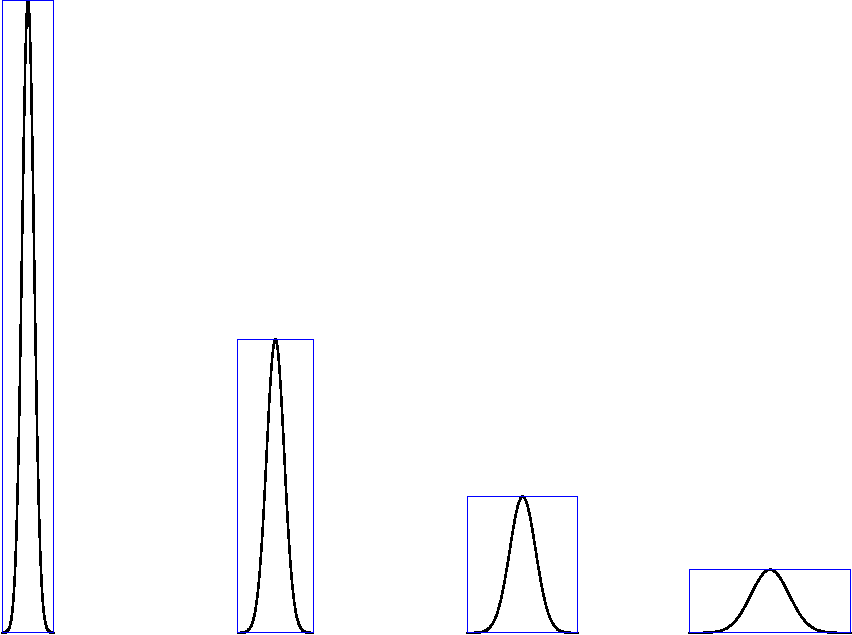
\includegraphics[width=0.5\textwidth]{heatscaling}

\emph{increasing time} \Large $\to$
\end{center}
\end{frame}


\begin{frame}{similarity solutions}

\begin{itemize}
\item Green's function of heat equation in 1D is
	$$T(t,x) = C\, t^{-1/2} e^{-x^2/(4Dt)}$$
\item ``similarity'' variables for 1D heat equation are
	$$s \stackrel{\text{\emph{input scaling}}}{\phantom{\Big|}=\phantom{\Big|}} t^{-1/2} x, \qquad T(t,x) \stackrel{\text{\emph{output scaling}}}{\phantom{\Big|}=\phantom{\Big|}} t^{-1/2} \phi(s)$$
\end{itemize}
\begin{columns}
\begin{column}{0.6\textwidth}
\begin{itemize}
\item \emph{historical note}:  in 1905 Einstein saw that the average distance traveled by particles in thermal motion scales like $\sqrt{t}$, so $s = t^{-1/2}x$ is an invariant
\end{itemize}
\end{column}
\begin{column}{0.4\textwidth}
\begin{center}
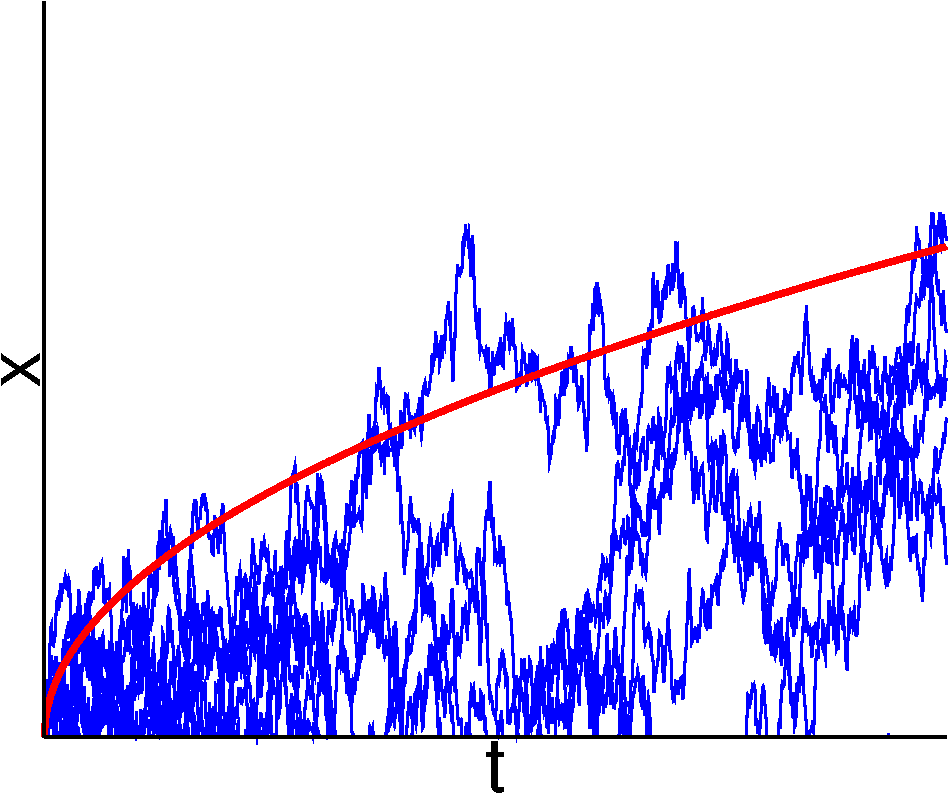
\includegraphics[width=1.0\textwidth]{brownian}
\end{center}
\end{column}
\end{columns}

\end{frame}


\subsection{solving the SIA}

\begin{frame}{similarity solution to SIA}

\begin{itemize}
\item jump forward to 1981
\item P.~Halfar found the similarity solution of the SIA in the case of flat bed and no surface mass balance \nocite{Halfar81,Halfar83}
\item Halfar's 2D solution for Glen flow law with $n=3$ has scalings
   $$H(t,r)=t^{-1/9} \phi(s), \qquad s = t^{-1/18} r$$
\item \dots so the diffusion of ice really slows down as the shape flattens out!
\end{itemize}
\end{frame}


\begin{frame}{Halfar solution to the SIA: the movie}
\label{slide:plothalfar}

\animategraphics[autoplay,loop,height=7.0cm]{4}{anim/halfar}{0}{26}

\par
\scriptsize 
frames from $t=4$ months to $t = 10^6$ years, equal spaced in \emph{exponential} time
\end{frame}


\begin{frame}{Halfar solution to the SIA: the formula}

\begin{itemize}
\item for $n=3$ the solution formula is:
  $$H(t,r) = H_0 \left(\frac{t_0}{t}\right)^{1/9} \left[1 - \left(\left(\frac{t_0}{t}\right)^{1/18} \frac{r}{R_0}\right)^{4/3}\right]^{3/7}$$
\item the ``characteristic time'' is
  $$t_0 = \frac{1}{18 \Gamma} \left(\frac{7}{4}\right)^3 \frac{R_0^4}{H_0^{7}}$$
if $H_0$, $R_0$ are central height and ice cap radius at $t=t_0$
\item you choose $H_0$ and $R_0$ and then determine $t_0$
\item it is a simple formula to use for verification!
\end{itemize}
\end{frame}


\begin{frame}{is the Halfar solution \emph{good for any modeling}?}

\begin{itemize}
\item John Nye and others (2000)\nocite{NyeIcarus2000} compared different flow laws for the South Polar Cap on Mars
\item they evaluated $\text{CO}_2$ ice and $\text{H}_2\text{O}$ ice softness parameters by comparing the long-time behavior of the corresponding Halfar solutions
\item conclusions:
  \begin{quote}
  \dots none of the three possible [$\text{CO}_2$] flow laws will allow a 3000-m cap, the thickness suggested by stereogrammetry, to survive for $10^7$ years, indicating that the south polar ice cap is probably not composed of pure $\text{CO}_2$ ice \dots the south polar cap probably consists of water ice, with an unknown admixture of dust.
  \end{quote}
\end{itemize}

\end{frame}


\begin{comment}
\begin{frame}{on ``degenerate'' diffusivity}

\begin{itemize}
\item recall that the SIA is
\small
	$$H_t = M + \Div \left(D\, \grad h \right) \quad \text{where} \quad D = \Gamma H^{n+2} |\grad h|^{n-1}$$
\normalsize
\item thus the diffusivity ``degenerates'', $D \to 0$, when either $H\to 0$ or $\grad h \to 0$
\item summary:
\small
\begin{tabular}{l|c|c}
 & why $D\to 0$ & so what? \\ \hline
domes    & $\grad h \to 0$ & \begin{tabular}{c}
$H$ and $\grad h$ are continuous \\ but $\grad^2 h$ is singular
\end{tabular} \\ \hline
margins  & $H \to 0$       & \begin{tabular}{c}
$H$ is continuous \\ but $\grad h$ is singular
\end{tabular}
\end{tabular}
\normalsize
\item in terms of numerical error, margin is worse than dome
\item degenerate diffusion equations are automatically free boundary problems
\end{itemize}
\end{frame}
\end{comment}

\begin{frame}
  \frametitle{computing diffusivity in SIA}

\begin{itemize}
\item for numerical stability we compute $D = \Gamma H^{n+2} |\grad h|^{n-1}$ on the staggered grid
\item various schemes proposed \small (Mahaffy, 1976\nocite{Mahaffy}; van der Veen 1999\nocite{vanderVeen}; Hindmarsh and Payne 1996\nocite{HindmarshPayne})
\item all schemes involve
  \begin{itemize}
  \item[$\circ$] averaging $H$
  \item[$\circ$] differencing $h$
  \item[$\circ$] in a ``balanced'' way, for better accuracy,
  \end{itemize}
to get the diffusivity on staggered grid
\end{itemize}

\begin{columns}
\begin{column}{0.65\textwidth}
\begin{itemize}
\item Mahaffy stencil \large $\to$ \normalsize
\end{itemize}
\end{column}

\begin{column}{0.35\textwidth}
  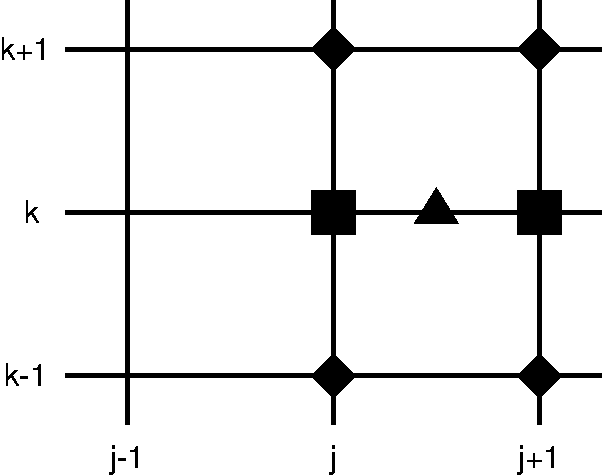
\includegraphics[width=1.0\textwidth]{mahaffystencil}
\end{column}
\end{columns}
\end{frame}


\begin{frame}
  \frametitle{SIA implementation: flat bed case}

\minputtiny{siaflat}

\end{frame}


\begin{frame}[fragile]
\frametitle{verifying SIA code vs Halfar}
\label{slide:verifysia}

\begin{columns}
\begin{column}{0.6\textwidth}
\scriptsize
\begin{verbatim}
octave:40> verifysia(20)
average abs error            = 22.310
maximum abs error            = 227.849
octave:41> verifysia(40)
average abs error            = 9.490
maximum abs error            = 241.470
octave:42> verifysia(80)
average abs error            = 2.800
maximum abs error            = 155.796
octave:43> verifysia(160)
average abs error            = 1.059
maximum abs error            = 109.466
\end{verbatim}
\normalsize

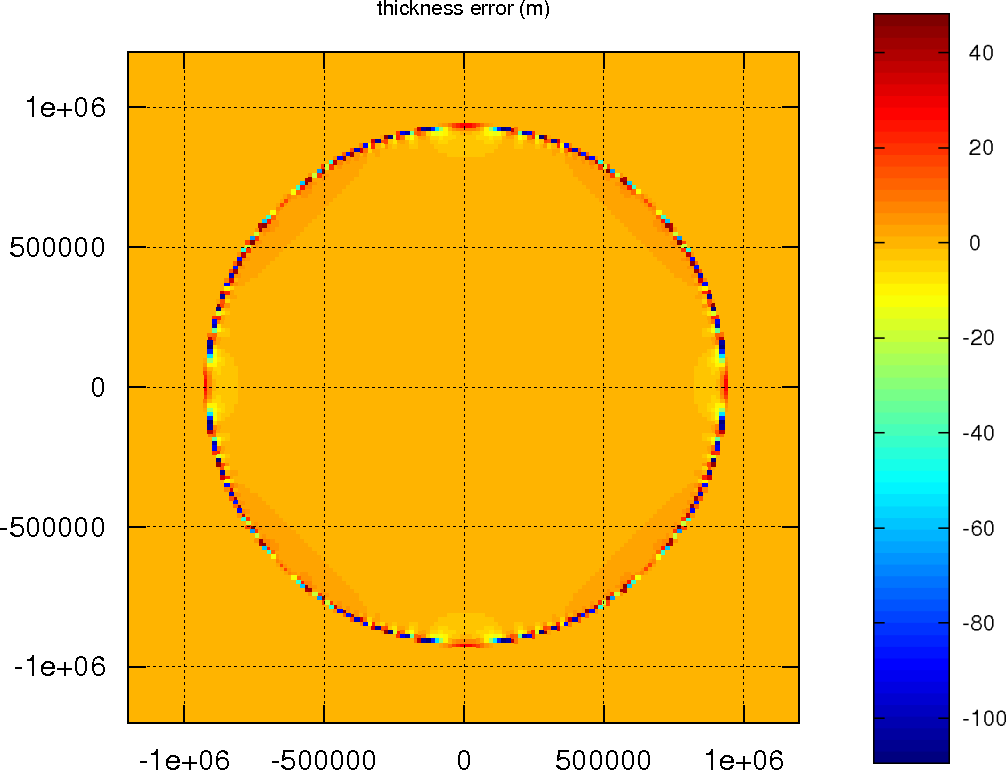
\includegraphics[width=0.8\textwidth]{siaerror}
\end{column}

\begin{column}{0.4\textwidth}
\small
\emph{Trust but verify.}
\medskip

\scriptsize
(Ronald Reagan)

\bigskip\bigskip\bigskip

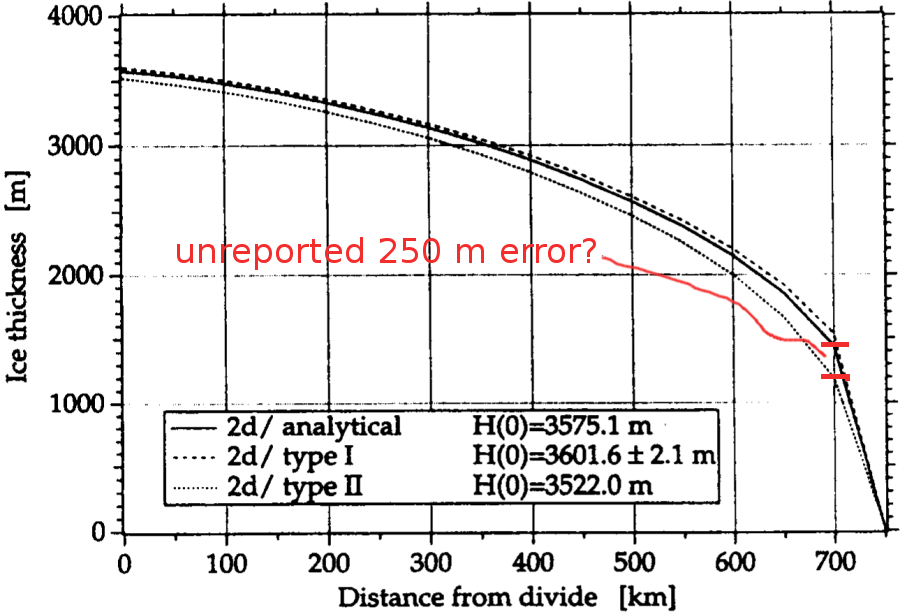
\includegraphics[width=1.0\textwidth]{eismintone}

\scriptsize \emph{figure 2 in Huybrechts et al.~(1996)}\nocite{EISMINT96}
\end{column}
\end{columns}
\end{frame}


\begin{frame}{demonstrate robustness}

see \texttt{roughice.m}, which calls \texttt{siaflat.m} after setting-up the nasty initial state at left:
\medskip

\begin{columns}
\begin{column}{0.5\textwidth}
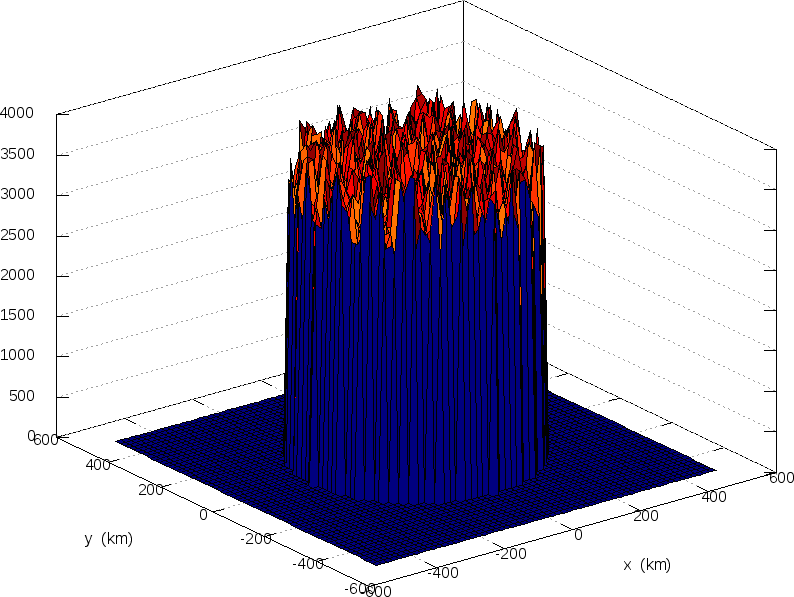
\includegraphics[width=1.0\textwidth]{roughinitial}
\end{column}
\begin{column}{0.5\textwidth}
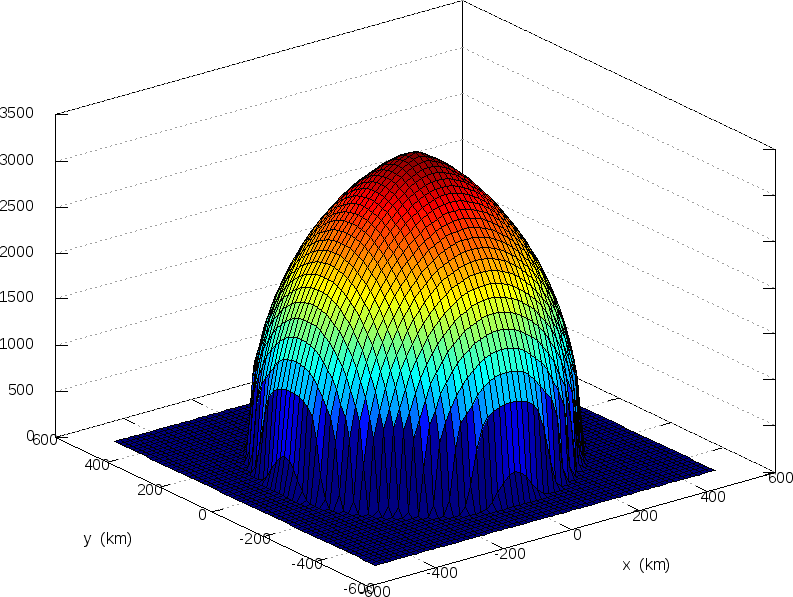
\includegraphics[width=1.0\textwidth]{roughfinal}
\end{column}
\end{columns}

\begin{center}
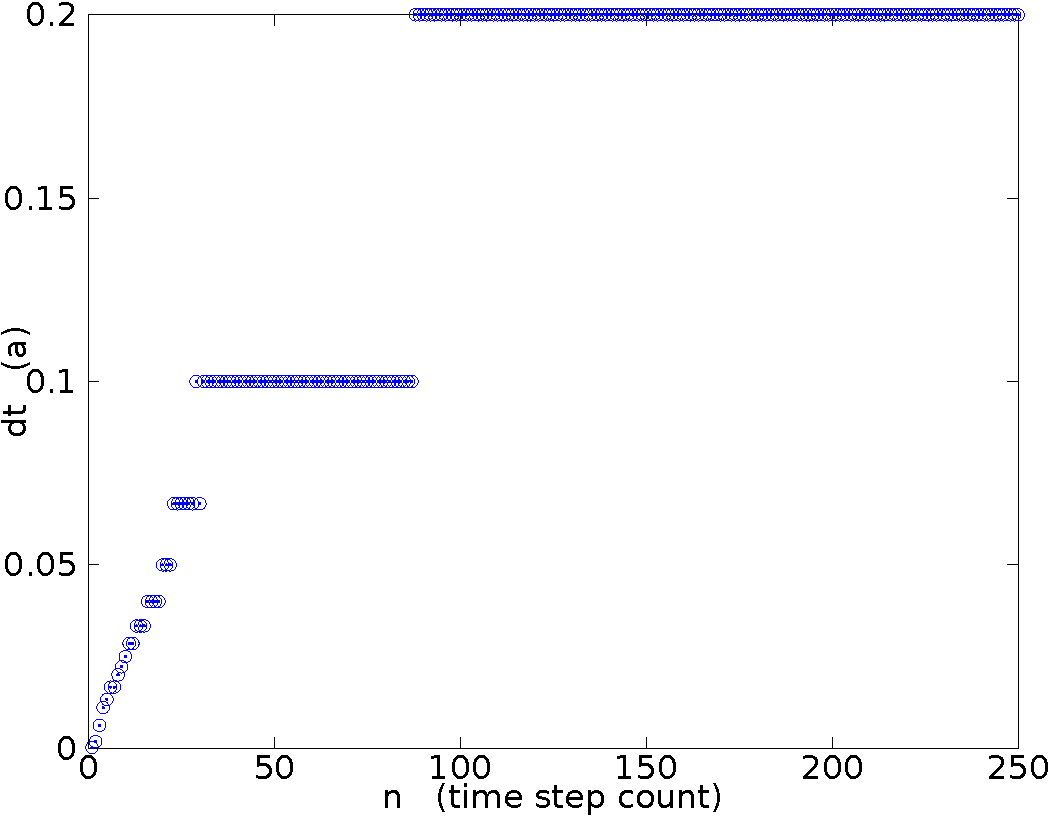
\includegraphics[width=0.4\textwidth]{roughtimesteps}
\end{center}
\end{frame}


\begin{frame}{model the Antarctic ice sheet}

\normalsize
\begin{itemize}
\item with careful-but-small modifications of \texttt{siaflat.m}, which make a good exercise:
  \begin{itemize}
  \item[$\circ$] observed accumulation as surface mass balance,
  \item[$\circ$] allow non-flat bed (so $H\ne h$),
  \item[$\circ$] compute surface slopes correctly where floating, and
  \item[$\circ$] calve at current calving front location
  \end{itemize}
here are results from this \emph{toy} Antarctic flow model
\item a 2000 model year run on a $\Delta x=50$ km grid; runtime a few seconds
\end{itemize}

\bigskip

\begin{columns}
\begin{column}{0.4\textwidth}
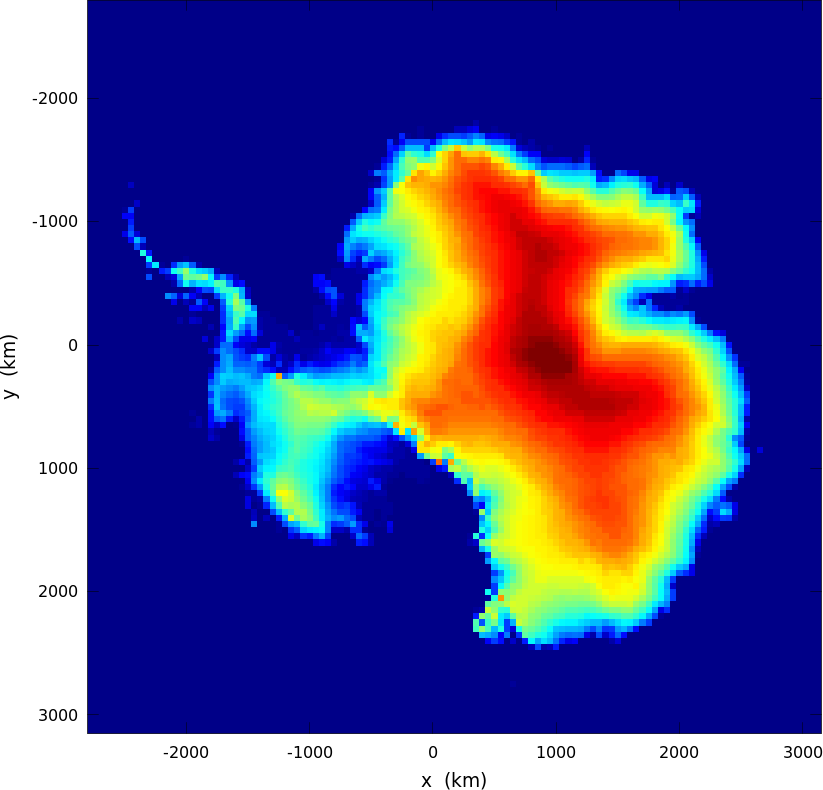
\includegraphics[height=1.75in]{antinitial}
\end{column}
\begin{column}{0.55\textwidth}
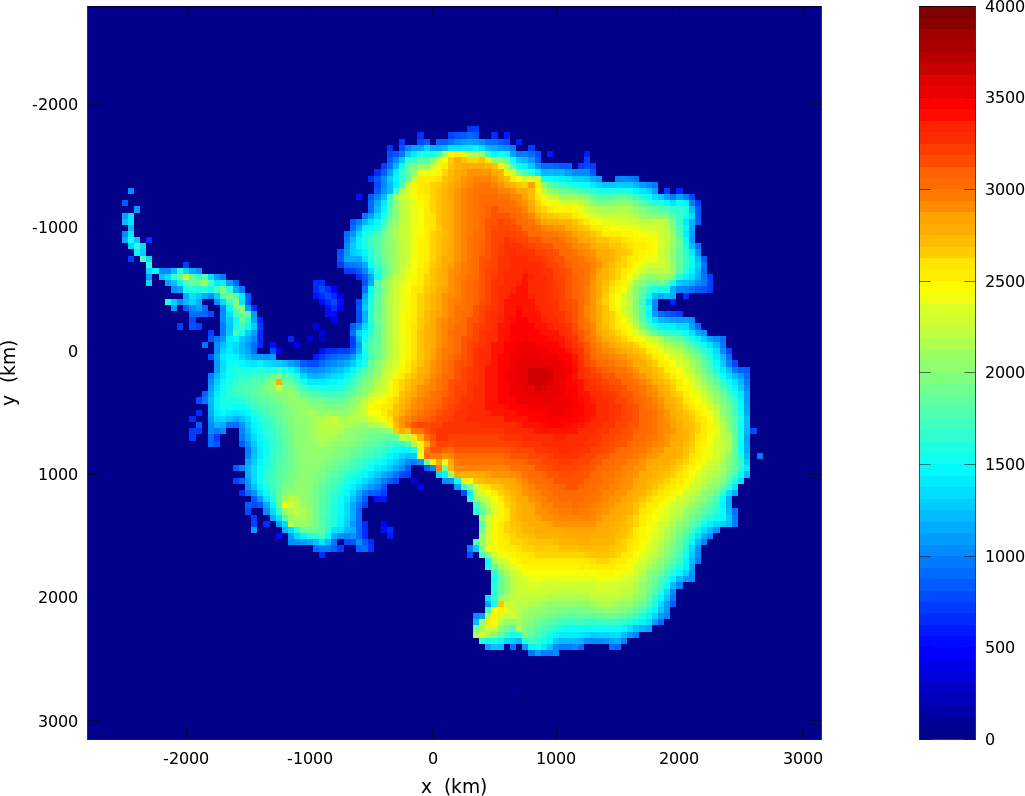
\includegraphics[height=1.75in]{antfinal}
\end{column}
\end{columns}
\end{frame}


\begin{comment}
\begin{frame}{final comments on SIA: origin and rigor}

where does the ``shallow ice approximation'' come from?:
\bigskip

\begin{itemize}
\item historically, Fowler and Larson (1978)\nocite{FowlerLarson1978}, Morland and Johnson (1980)\nocite{MorlandJohnson}, and Hutter (1983)\nocite{Hutter} \dots thus recent
\item logically, by a ``small-parameter argument'', based on a small depth-to-width ratio, from the more complete Stokes model for slow ice flow
\item more precisely, by using the small aspect ratio \, $\eps = [H]/[L]$ \, of ice sheets to scale the Stokes model to see which terms make small contributions
\end{itemize}
\end{frame}
\end{comment}



\section{mass continuity}

\begin{frame}{the most basic shallow assumption}

\begin{columns}

\begin{column}{0.6\textwidth}
\begin{itemize}
\item there are many shallow theories: SIA, SSA, hybrids, Blatter, \dots
\item \emph{all} make one assumption not required in Stokes:

\begin{center}
\alert{the surface and base of the ice are given by functions $z=h(t,x,y)$ and $z=b(t,x,y)$}
\end{center}
\item surface overhang is not allowed
\item most Stokes models make this assumption too?
\end{itemize}
\end{column}

\begin{column}{0.4\textwidth}
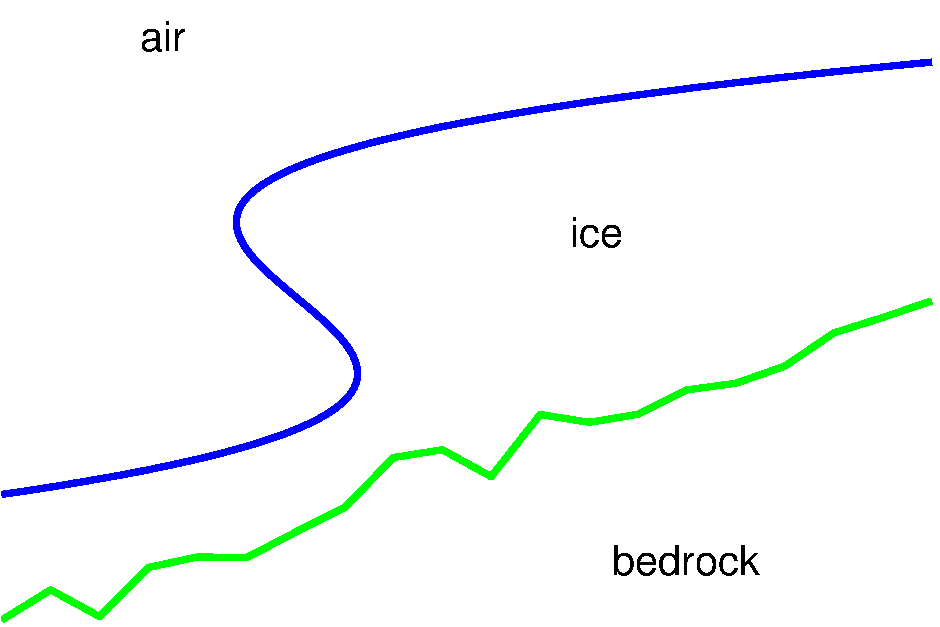
\includegraphics[width=1.0\textwidth]{sshape}

\scriptsize
\begin{center}
\emph{not shallow!}
\end{center}
\vspace{6mm}

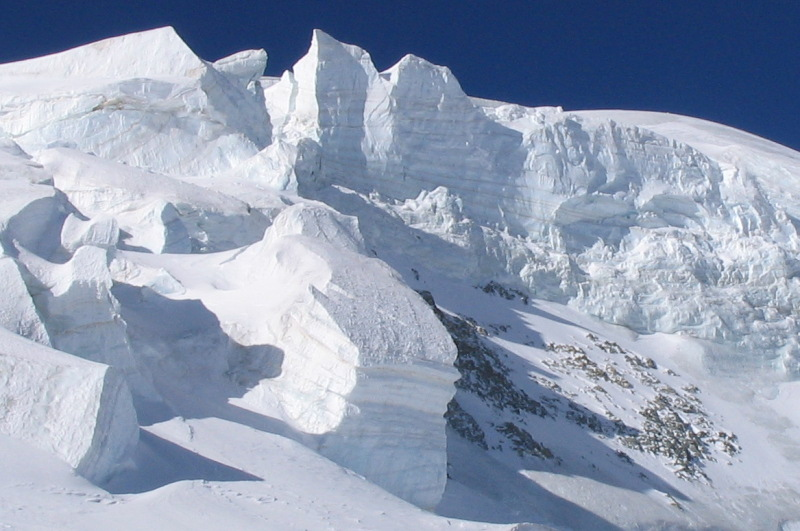
\includegraphics[width=1.0\textwidth]{serac}

\begin{center}
\emph{not shallow!}
\end{center}
\end{column}
\end{columns}
\end{frame}


\begin{frame}{three equations for geometry change}

\begin{itemize}
\item let $a$ be the climatic (surface) mass balance function;  $a>0$ is accumulation
\item $s$ be the basal melt rate function;  $s>0$ is basal melting
\item let $M=a-s$: ``climatic-basal mass balance function'' in glossary
\item define the map-plane flux of ice,
	$$\bq = \int_{b}^{h} (u,v)\,dz = \overline{\mathbf{U}}\,H$$
\item the three equations for geometry change:
\begin{align*}
&\text{surface kinematical} && h_t = a - u\big|_h h_x - v\big|_h h_y + w\big|_h  \\
&\text{base kinematical} && b_t = s - u\big|_b b_x - v\big|_b b_y + w\big|_b  \\
&\text{mass continuity} && H_t = M - \Div \bq \\
\end{align*}
\end{itemize}
\end{frame}


\begin{frame}{kinematic and mass continuity equations}

\begin{itemize}
\item what does the ``most basic shallow assumption'' get you?
\item \emph{answer 1}: a (map-plane) mass continuity equation from the kinematical equations and incompressibility
\item \emph{answer 2}: of these three equations,
  \begin{itemize}
  \item[$\circ$]  surface kinematical
  \item[$\circ$]  base kinematical
  \item[$\circ$]  mass continuity
  \end{itemize}
\emph{any two imply the third}

\bigskip
\item to show the above, recall:
  \begin{itemize}
  \item[$\circ$]  the incompressibility of ice
    $$u_x + v_y + w_z = 0$$
  \item[$\circ$]  and the Leibniz rule for differentiating integrals
  \scriptsize
    $$\frac{d}{dx}\left(\int_{g(x)}^{f(x)} h(x,y)\,dy\right) = f'(x) h(x,f(x)) - g'(x) h(x,g(x)) + \int_{g(x)}^{f(x)} h_x(x,y)\,dy$$
  \end{itemize}
\end{itemize}
\end{frame}


\begin{frame}{kinematic and mass continuity equations 2}

\begin{itemize}
\item literature is full of incomplete calculations of these equivalences
\item \dots usually mixed in with small-parameter arguments about shallowness
\item most ice sheet models use the mass continuity equation
\item \dots but they could instead use the surface kinematical equation
\end{itemize}
\end{frame}


\begin{frame}{standard recipe for ice sheet models}

\begin{itemize}
\item the ingredients of a typical ice sheet model:
  \begin{enumerate}
  \item numerical implementation of a stress balance: compute velocity $(u,v,w)$
  \item from the horizontal velocity $(u,v)$ and the surface balance, do time-step of mass continuity equation to get $H_t$
  \item update surface elevation (and bed elevation)
  \item decide on time-step, and repeat at 1.
  \end{enumerate}
\end{itemize}
\end{frame}



\section{shelves and streams}


\subsection{shallow shelf aprx (SSA)}

\begin{frame}{flow model II: shallow shelf approximation (SSA) stress balance}
  
SSA model applies very well to \alert{ice shelves}
\begin{itemize}
\item \dots for parts away from grounding lines
\item \dots and away from calving fronts
\end{itemize}

\bigskip\bigskip

\begin{center}
  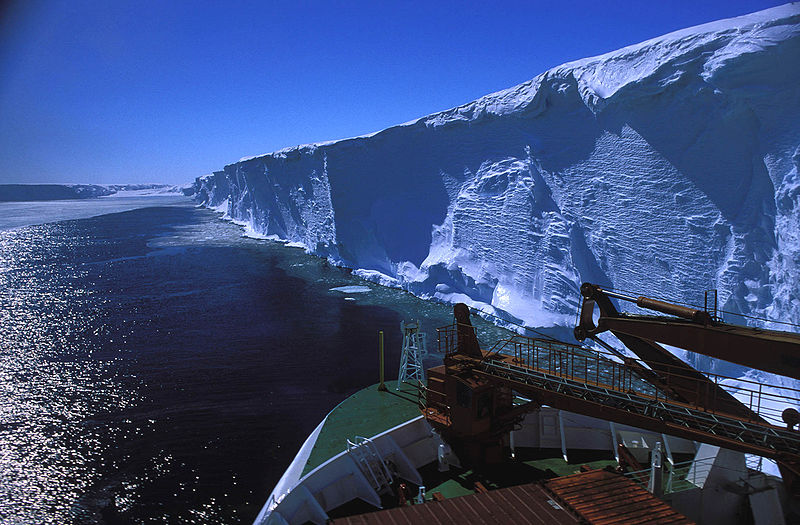
\includegraphics[width=0.6\textwidth]{iceshelfedge}

\tiny Ekstr\"om ice shelf(Hans Grobe)
\end{center}
\end{frame}


\begin{frame}{shallow shelf approximation stress balance 2}

SSA also applies reasonably well to \alert{ice streams}
\begin{itemize}
\item \dots with modest bed topography
\item \dots and weak bed strength\footnote{energy conservation (esp.~ice temperature and basal melt) and subglacial hydrology (esp.~subglacial water pressure) are major aspects of ice stream flow \dots but not addressed here}
\item imperfect near shear margins and grounding lines
\end{itemize}

\begin{center}
  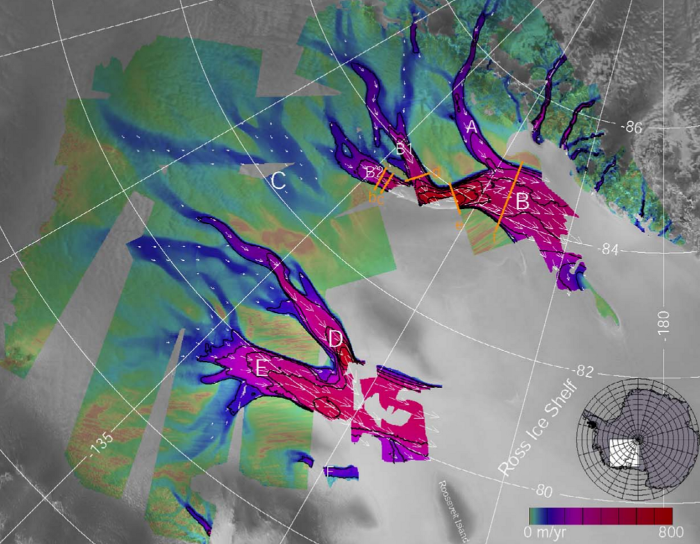
\includegraphics[width=0.6\textwidth]{siple}

\tiny surface velocity for Siple Coast ice streams, Antarctica 
\end{center}
\end{frame}


\begin{frame}{what is, \emph{and is not}, an ice stream?}

\begin{columns}
\begin{column}{0.6\textwidth}
\begin{itemize}
\item ice streams 
  \small
  \begin{itemize}
  \item[$\circ$] slide ($100$ to $1000 \,\text{m}\,\text{a}^{-1}$)
  \item[$\circ$] have concentrated vertical shear in thin layer near base
  \end{itemize}
  \normalsize
\item ``outlet glaciers''
  \begin{itemize}
  \item[$\circ$] fast surface speed (up to $10 \,\text{km}\,\text{a}^{-1}$)
  \item[$\circ$] uncertain how much is sliding
  \item[$\circ$] substantial vertical shear ``up'' in the ice column,
  \item[$\circ$] not-at-all flat bed topography
  \item[$\circ$] soft, temperate ice may play a big role
  \end{itemize} 
\item \alert{few simplifying assumptions are appropriate for outlet glaciers}
\end{itemize}
\end{column}

\begin{column}{0.4\textwidth}
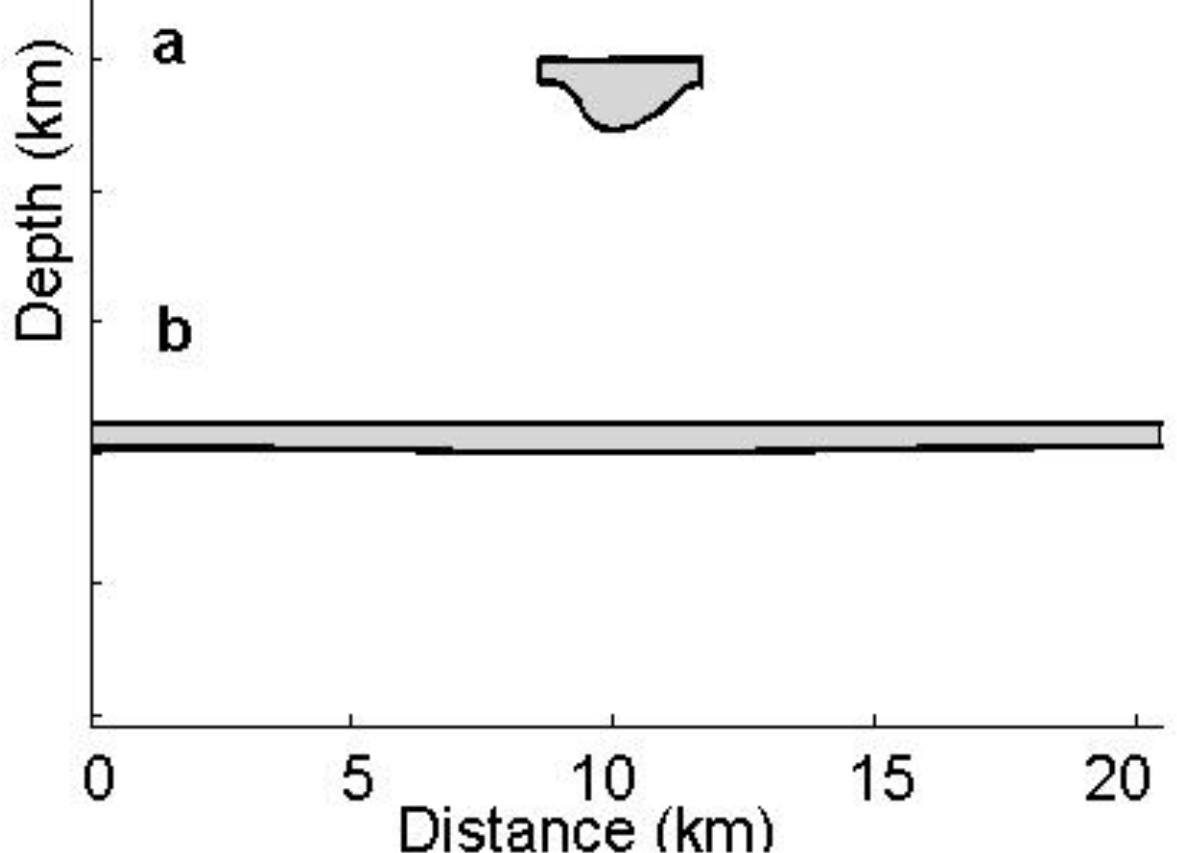
\includegraphics[width=1.0\textwidth]{streamisbrae}

\bigskip
\scriptsize 
Jakobshavns Isbrae (\textbf{a}) and Whillans Ice Stream (\textbf{b}); plotted without vertical exaggeration (\tiny Truffer and Echelmeyer (2003), \emph{Of isbrae and ice streams}\scriptsize)
\end{column}
\end{columns}
\end{frame}


\begin{frame}{SSA stress balance equation}

\begin{itemize}
\item only plane flow case (``flow line'') here
\item the stress balance equation which determines velocity in an \emph{ice stream}:
\begin{empheq}[box=\fbox]{equation}
  \left({\color{red}2 A^{-1/n} H |u_x|^{1/n - 1} u_x}\right)_x - {\color{blue}C|u|^{m-1}u} = {\color{green}\rho g H h_x} \label{ssa}
\end{empheq}
\item the {\color{red} red term} inside parentheses is the vertically-integrated ``longitudinal'' or ``membrane'' stress
\item the {\color{blue} blue term} is basal resistance
\item the {\color{green} green term} is  driving stress
\item derived originally by Morland (1987), MacAyeal (1989)
\item \emph{how to think about this equation}?
\item \emph{how do you solve it numerically}?
\end{itemize}
\end{frame}


\begin{frame}{flow line model: from stream to shelf}
\label{slide:streamtoshelf}

\small
\begin{align*}
  u = u_0 & \qquad \text{ at } x = 0 \\
  \left.\begin{array}{r}
  \left(2 A^{-1/n} H |u_x|^{1/n - 1} u_x\right)_x - C|u|^{m-1}u = \rho g H h_x \\
  h = H + b
  \end{array}\right\}& \qquad \text{ on } 0 < x < x_g \\
  \left.\begin{array}{r}
  \left(2 A^{-1/n} H |u_x|^{1/n - 1} u_x\right)_x + 0 = \rho g H h_x \\
  h = (1-\rho/\rho_w) H
  \end{array}\right\}& \qquad \text{ on } x_g < x < x_c \\
  2 A^{-1/n} H |u_x|^{1/n - 1} u_x = \frac{1}{2}\rho (1-\rho/\rho_w) g H^2 & \qquad \text{ at } x = x_c
\end{align*}

\bigskip\bigskip
\begin{center}
  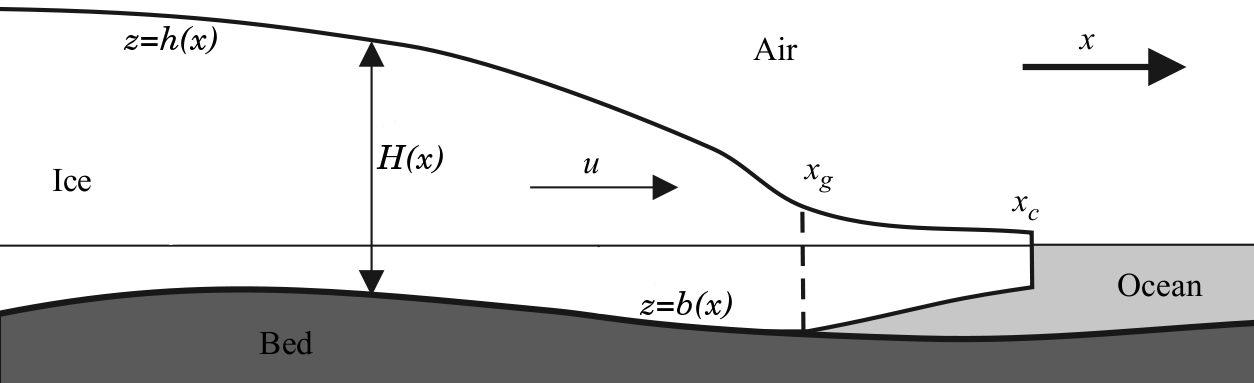
\includegraphics[width=0.7\textwidth]{flowline}
\end{center}
\end{frame}


\begin{frame}{flotation criterion and grounding line}

\begin{itemize}
\item the inequality ``$\rho H < - \rho_w b$'' is the \alert{flotation criterion}
\item at the grounding line $x=x_g$ the above inequality switches
\item \dots and the driving stress switches form:
  \begin{itemize}
  \item[$\circ$] on the grounded side we know $\rho H > - \rho_w b$ so
  	$$\rho g H h_x = \rho g H (H_x + b_x)$$
  \item[$\circ$] on the floating side we know $\rho H < - \rho_w b$ so $h = (1-\rho/\rho_w) H$ and so
  	$$\rho g H h_x = \rho(1-\rho/\rho_w) g H H_x$$
  \end{itemize}
\item also: $H,u,u_x$ are all continuous at $x=x_g$
\end{itemize}
\end{frame}



\subsection{ice shelf flow line solution}


\begin{frame}{exact velocity and thickness for steady ice shelf}

\begin{itemize}
\item limited goal here: describe a steady state, 1D ice shelf
\item there is a nice \alert{by-hand} result (next slide): the thickness and velocity in the ice shelf can be completely determined in terms of the 
  \begin{enumerate}
  \item ice thickness $H_g$ at the grounding line and
  \item ice velocity $u_g$ at the grounding line
  \end{enumerate}
\item we will use this to
  \begin{itemize}
  \item[$\circ$] understand the SSA better
  \item[$\circ$] verify a numerical SSA code
  \end{itemize}
\end{itemize}
\end{frame}


\begin{frame}{exact velocity and thickness for steady ice shelf 2}

\small see \texttt{testshelf.m} 

\begin{center}
  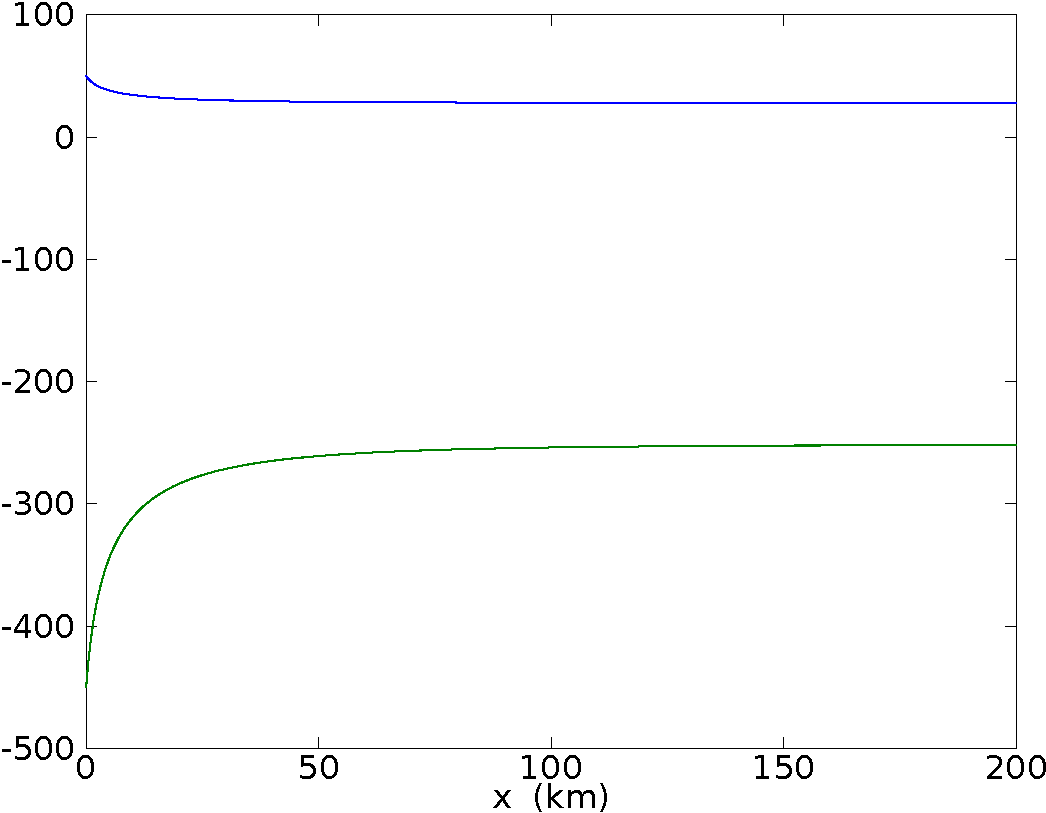
\includegraphics[width=0.45\textwidth]{steadyshelfprofile} \quad
  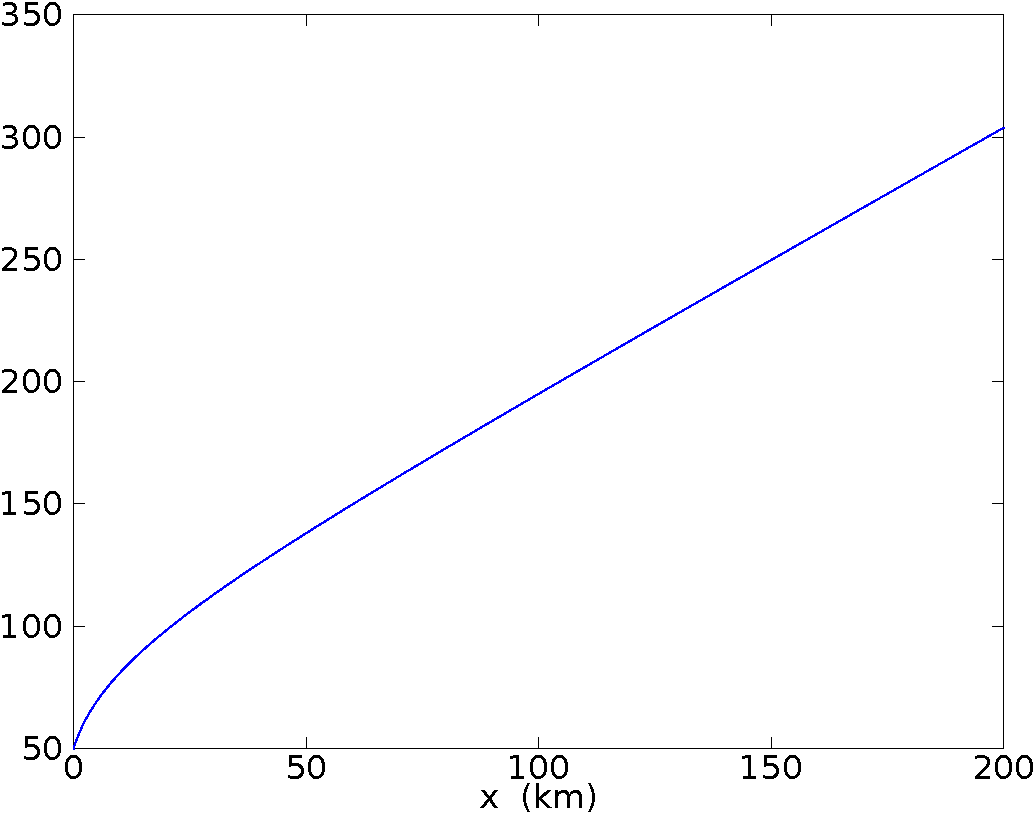
\includegraphics[width=0.45\textwidth]{steadyshelfvelocity}
\end{center}

\bigskip\bigskip

\includegraphics[width=0.3\textwidth]{rocket-nozzle-expansion}
\end{frame}


\subsection{numerical SSA}

\begin{frame}{numerically solving the SSA stress balance}

\begin{itemize}
\item here we fix ice thickness $H(x)$ and find the velocity numerically
\item the stress balance is a nonlinear equation in the velocity:
  $$\left(2 A^{-1/n} H |u_x|^{1/n - 1} u_x\right)_x - C|u|^{m-1}u = \rho g H h_x$$
\item \alert{iteration is needed}
\item I'll describe the numerical method for a shelf \emph{or} stream, but only give a code for an ice shelf
\end{itemize}
\end{frame}


\begin{frame}{numerically solving the SSA stress balance 2}

\begin{itemize}
\item coefficient ${\color{red} \bar \nu} = A^{-1/n} |u_x|^{1/n-1}$ is the ``effective viscosity'':
   $$\left(2 \,{\color{red} \bar \nu}\, H u_x\right)_x - C |u|^{m-1} u = \rho g H h_x$$
\item \emph{simplest iteration idea}: use old effective viscosity to get new velocity solution, and repeat until things stop changing
  \begin{itemize}
  \item[$\circ$] this is ``Picard'' iteration
  \item[$\circ$] Newton iteration is a superior alternative
  \end{itemize}
\item specifically:
  \begin{itemize}
  \item[$\circ$] last iterate $u^{(k-1)}$
  \item[$\circ$] define $W^{(k-1)} = 2 \bar \nu H = 2 A^{-1/n} |u^{(k-1)}_x|^{1/n-1} H$
  \item[$\circ$] current iterate (unknown) $u^{(k)}$
  \item[$\circ$] solve repeatedly:
     $$\left(W^{(k-1)} u^{(k)}_x\right)_x - C |u^{(k-1)}|^{m-1} u^{(k)} = \rho g H h_x$$
  \end{itemize}
\end{itemize}
\end{frame}


\begin{frame}{solving the ``inner'' linear problem}
\begin{itemize}
\item abstract the problem:
   $$\left(W(x)\, u_x\right)_x - \alpha(x)\, u = \beta(x)$$
on $0 < x < L$, with boundary conditions
   $$u(0) = V, \qquad  u_x(L) = \gamma$$
\item an \emph{elliptic} PDE boundary value problem
\item $W(x)$, $\alpha(x)$, $\beta(x)$ are known functions in the SSA context:
  \begin{itemize}
  \item[$\circ$] both $W(x)$ and $\alpha(x)$ come from previous iteration
  \item[$\circ$] $\beta(x)$ is driving stress
  \end{itemize}
\end{itemize}
\end{frame}


\begin{frame}{where do you get an initial guess $u^{(0)}$?}

\begin{itemize}
\item \emph{for floating ice}, a possible initial guess for velocity comes from assuming a uniform strain rate:
   $$u^{(0)}(x) = \gamma (x-x_g) + u_g$$
where $\gamma$ is the value of $u_x$ found from calving front stress imbalance
\item \emph{for grounded ice}, a possible initial guess for velocity is to assume ice is held by basal resistance only:
   $$u^{(0)}(x) = \left(-C^{-1} \rho g H h_x\right)^{1/m}$$
\end{itemize}
\end{frame}


\begin{frame}{numerics of the ``inner'' linear problem}

\begin{itemize}
\item suppose $j=1,2,\dots,J+1$, where $x_1 = x_g$ and $x_{J+1} = x_c$ are endpoints
\item $W(x)$ is needed on the staggered grid; the approximation is:
$$\frac{W_{j+1/2} (u_{j+1} - u_j) - W_{j-1/2} (u_{j} - u_{j-1})}{\Delta x^2} - \alpha_j u_j \stackrel{\ast}{=} \beta_j$$
\item left-hand boundary condition: $u_1 = V$ given
\item right-hand boundary condition (``$u_x(L)=\gamma$''):
  \begin{itemize}
  \item[$\circ$] introduce notional point $x_{J+2}$
  \item[$\circ$]
    $$\frac{u_{J+2} - u_J}{2 \Delta x} = \gamma$$
  \item[$\circ$] using equation $\ast$ in $j=J+1$ case, eliminate $u_{J+2}$ variable ``by-hand'' before coding numerics
  \end{itemize}
\end{itemize}
\end{frame}


\begin{frame}{numerics of the ``inner'' linear problem 2}

\scriptsize
\begin{itemize}
\item so SSA stress balance has form  \quad $A \mathbf{x} = \mathbf{b}$, \quad namely:
$$
\begin{bmatrix}
1 &  &  &  &  \\
W_{3/2} & A_{22} & W_{5/2} &  &  \\
 & W_{5/2} & A_{33} &  &  \\
 &  & \ddots & \ddots &  \\
 &  & W_{J-1/2} & A_{JJ} & W_{J+1/2} \\
 &  &  & A_{J+1,J} & A_{J+1,J+1} \\
\end{bmatrix}\,
\begin{bmatrix}
u_1 \\ u_2 \\ u_3 \\ \vdots \\ u_J \\ u_{J+1}
\end{bmatrix}
=
\begin{bmatrix}
0 \\ \beta_2 \Delta x^2 \\ \beta_3 \Delta x^2 \\ \vdots \\ \beta_J \Delta x^2 \\ b_{J+1}
\end{bmatrix}
$$
\item with diagonal entries
$$A_{22} = -(W_{3/2}+W_{5/2}+\alpha_1 \Delta x^2)$$
$$A_{33} = -(W_{5/2}+W_{7/2}+\alpha_2 \Delta x^2)$$
and so on, up to $A_{JJ}$, 
\item with special cases in last equation:
$$A_{J+1,J} = 2 W_{J+1/2}$$
$$A_{J+1,J+1} = -(2 W_{J+1/2}+\alpha_{J+1}\Delta x^2)$$
$$b_{J+1} = -2 \gamma \Delta x W_{J+3/2} + \beta_{J+1} \Delta x^2$$
\item this is a \emph{tridiagonal} system
\end{itemize}
\end{frame}


\begin{frame}{numerics of the ``inner'' linear problem 3}
\label{slide:flowlinecode}

\minput{flowline}
\end{frame}


\begin{frame}{testing the ``inner'' linear code}

\begin{itemize}
\item before proceeding to solve nonlinear SSA problem, we can test the ``abstracted'' code \texttt{flowline.m}
\item test by ``manufacturing'' solutions
  \begin{itemize}
  \item[$\circ$] see \texttt{testflowline.m}; not shown
  \end{itemize}
\item results:
  \begin{itemize}
  \item[$\circ$] converges at optimal rate $O(\Delta x^2)$
  \end{itemize}
\end{itemize}
\end{frame}


\begin{frame}{numerical: SSA}

\minputtiny{ssaflowline}
\end{frame}


\begin{frame}[fragile]
  \frametitle{\emph{numerical} thickness and velocity for steady ice shelf}

lines below are a convergence analysis of \texttt{testshelf.m}, which calls \texttt{ssaflowline.m}:

\begin{center}
  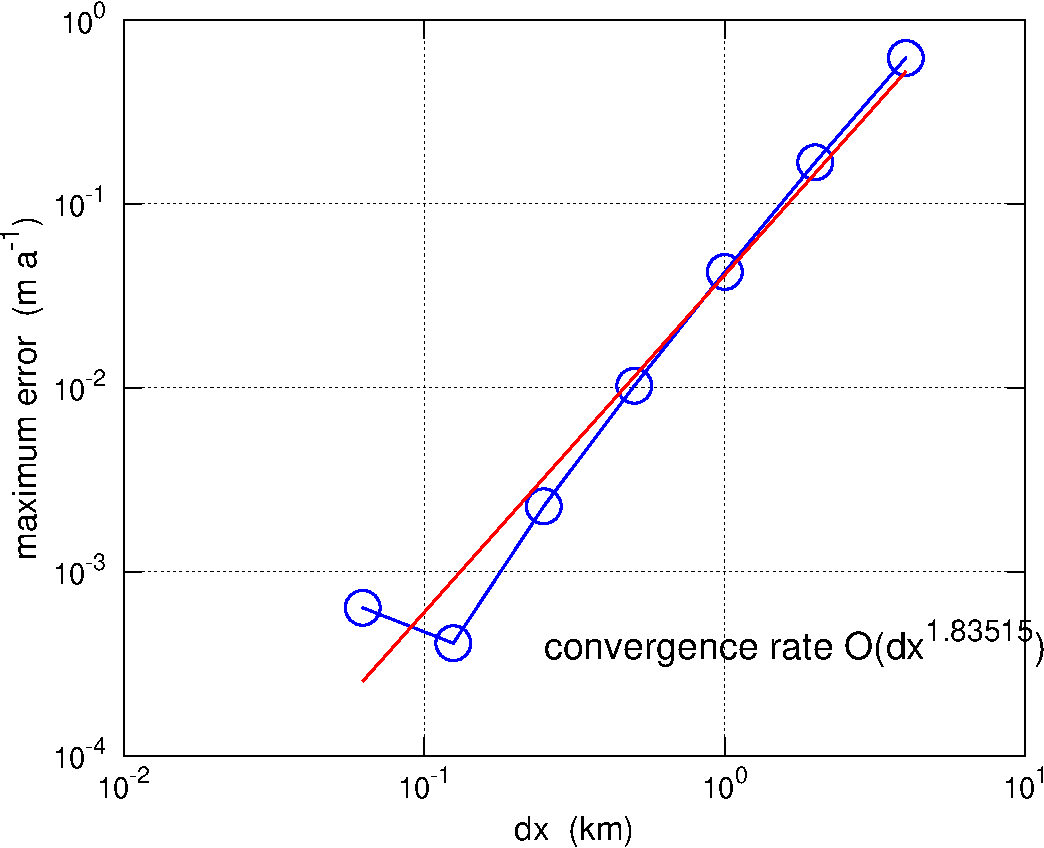
\includegraphics[width=0.75\textwidth]{shelfconv}
\end{center}
\end{frame}


\begin{frame}{SSA model output}

\begin{center}
  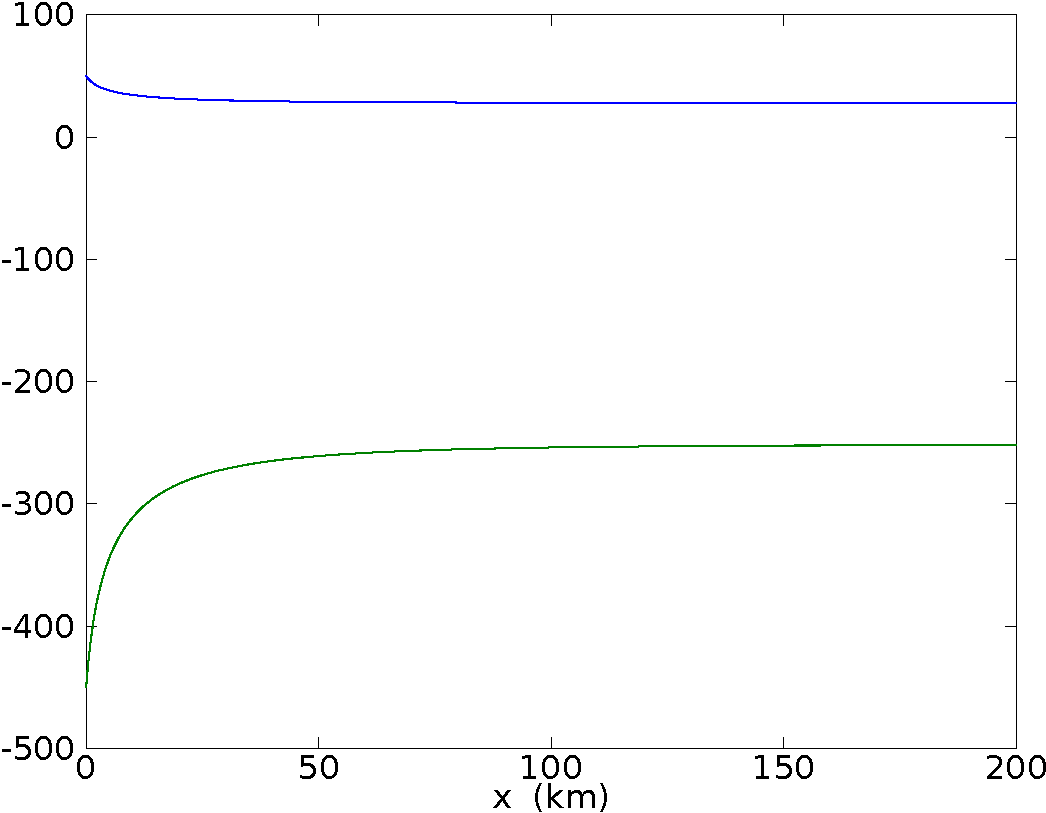
\includegraphics[width=0.45\textwidth]{steadyshelfprofile} \quad
  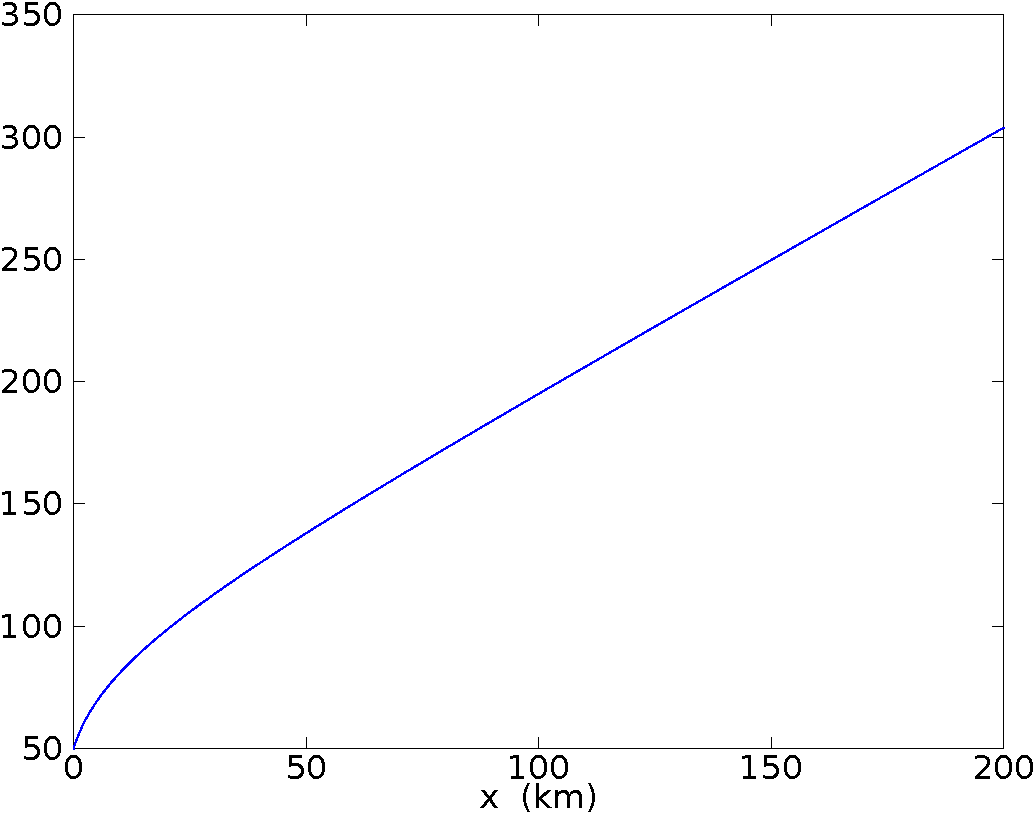
\includegraphics[width=0.45\textwidth]{steadyshelfvelocity}
\end{center}

\bigskip

\begin{itemize}
\item \emph{this looks suspiciously like figures for the exact solution \dots}
\item yes
\end{itemize}
\end{frame}


\begin{frame}{realistic ice shelf modeling}

\begin{itemize}
\item flow lines are never very realistic
\item you can add parameterized ``side drag'' \dots
\item also, ice shelves have surprises:
  \begin{itemize}
  \item[$\circ$] high basal melt near grounding lines
  \item[$\circ$] marine ice can freeze-on at bottom (below)
  \item[$\circ$] ``reverse slope'' bed instability and WAIS \dots
  \end{itemize}
\end{itemize}

\medskip
\begin{center}
  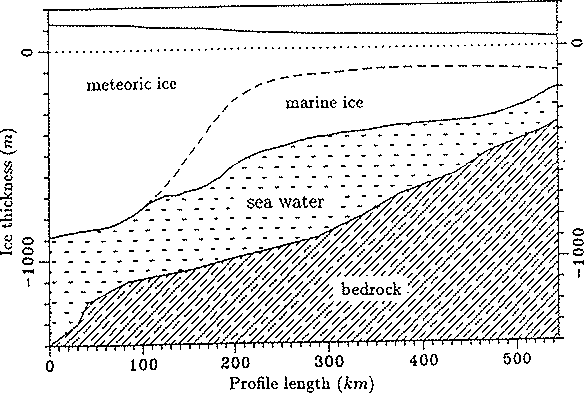
\includegraphics[width=0.5\textwidth]{marineice}
  
  \medskip
  \tiny from Grosfeld \& Thyssen 1994
\end{center}
\end{frame}


\begin{frame}{ice shelf modeling in 2D}

\begin{itemize}
\item nonetheless ``diagnostic'' (static geometry) ice shelf modeling in 2d has been quite successful
\item observed surface velocities validate SSA stress balance model
  \begin{itemize}
  \item[$\circ$] e.g.~Ross ice shelf example below using PISM
  \item[$\circ$] \dots but many models can do this
  \end{itemize}
\end{itemize}

\begin{center}
  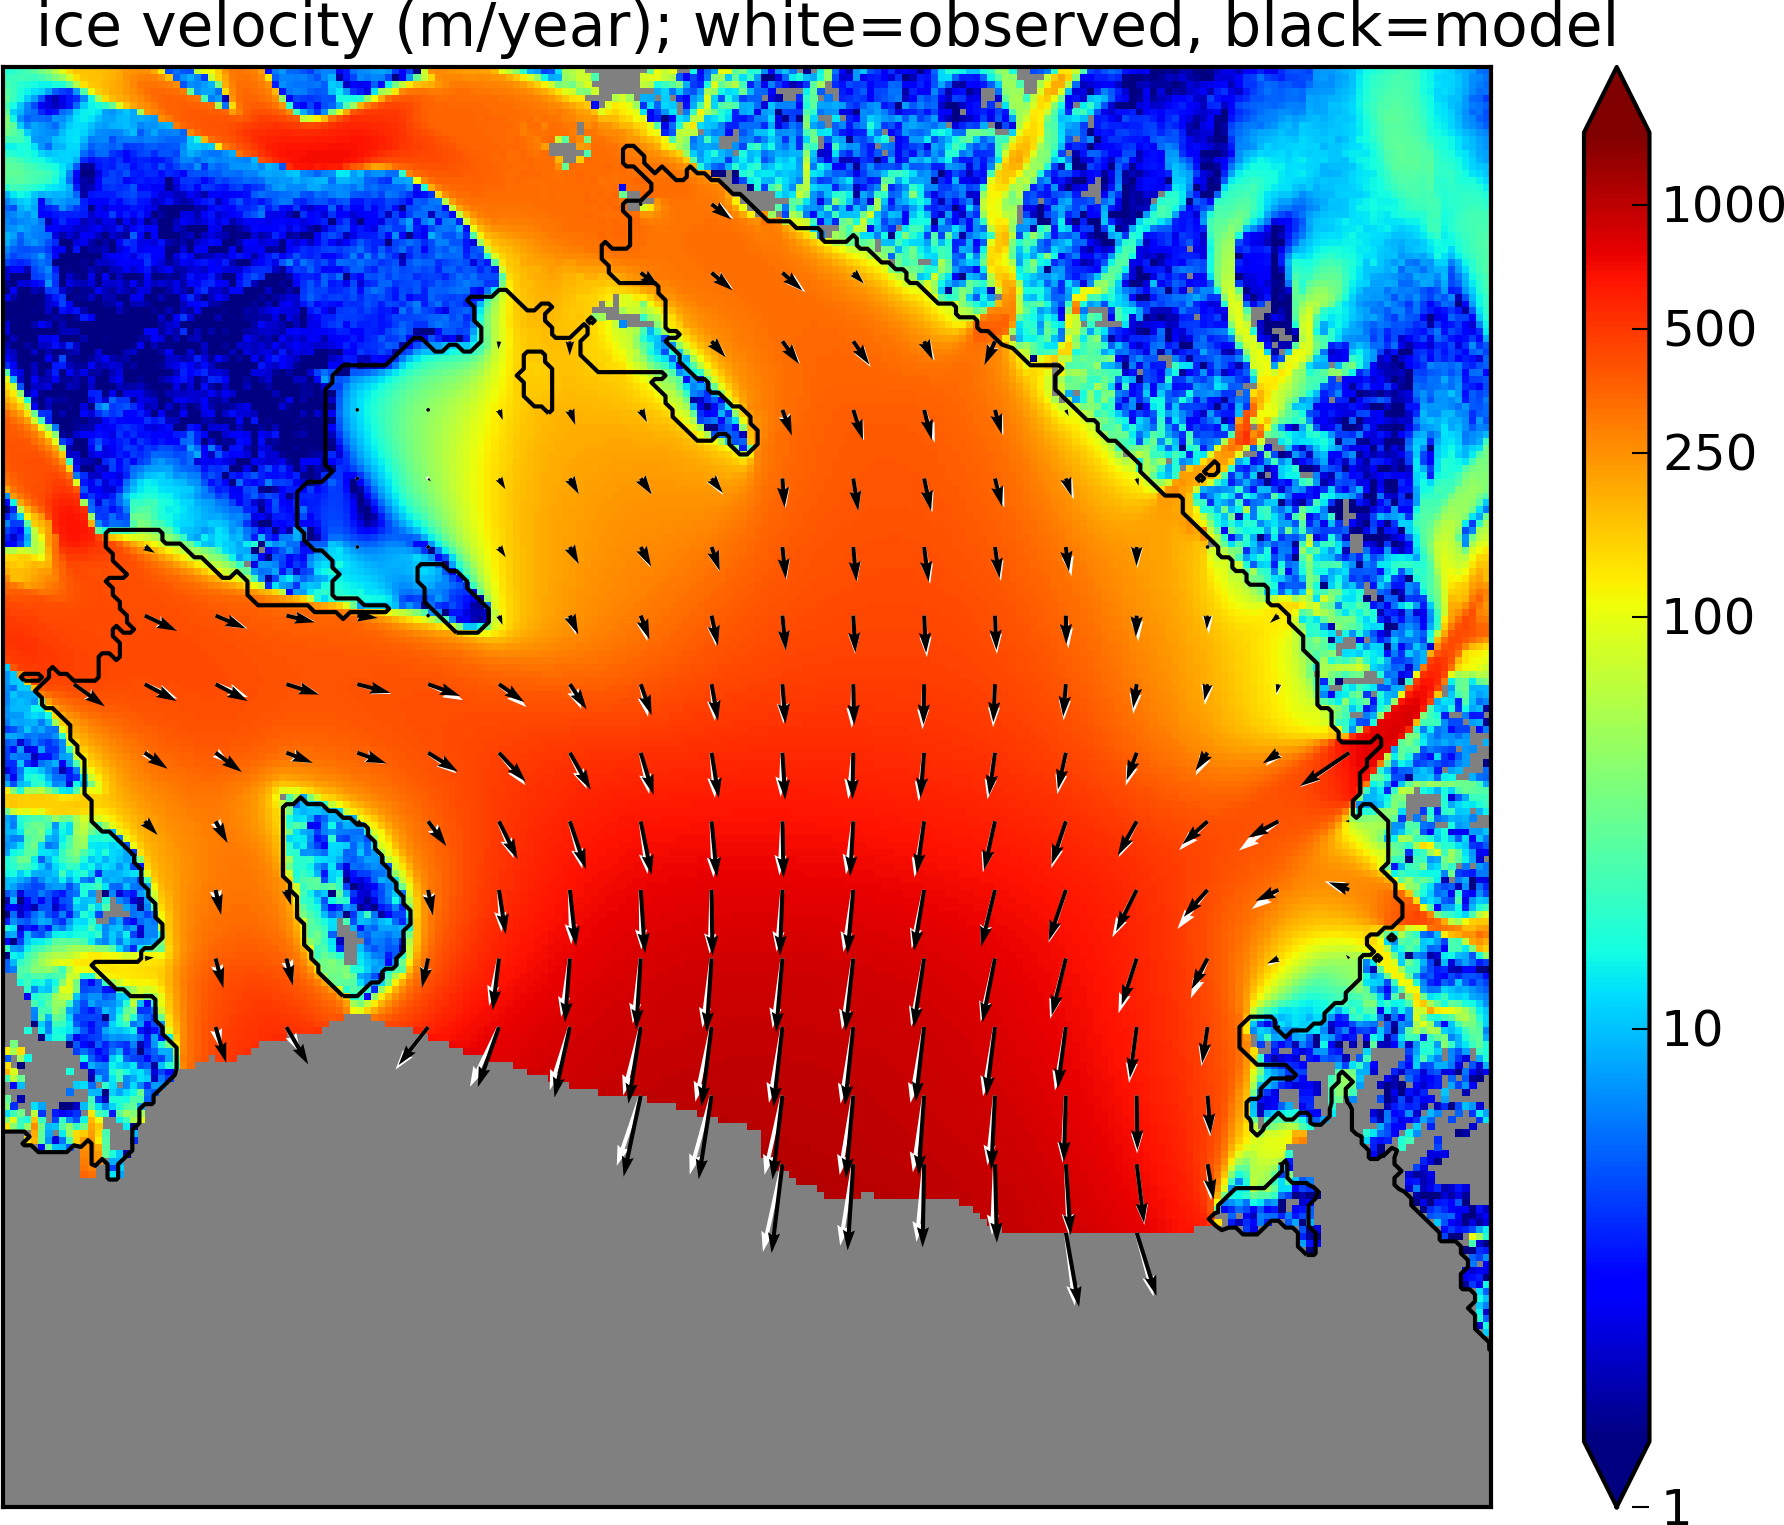
\includegraphics[width=0.5\textwidth]{rossquiver} \quad  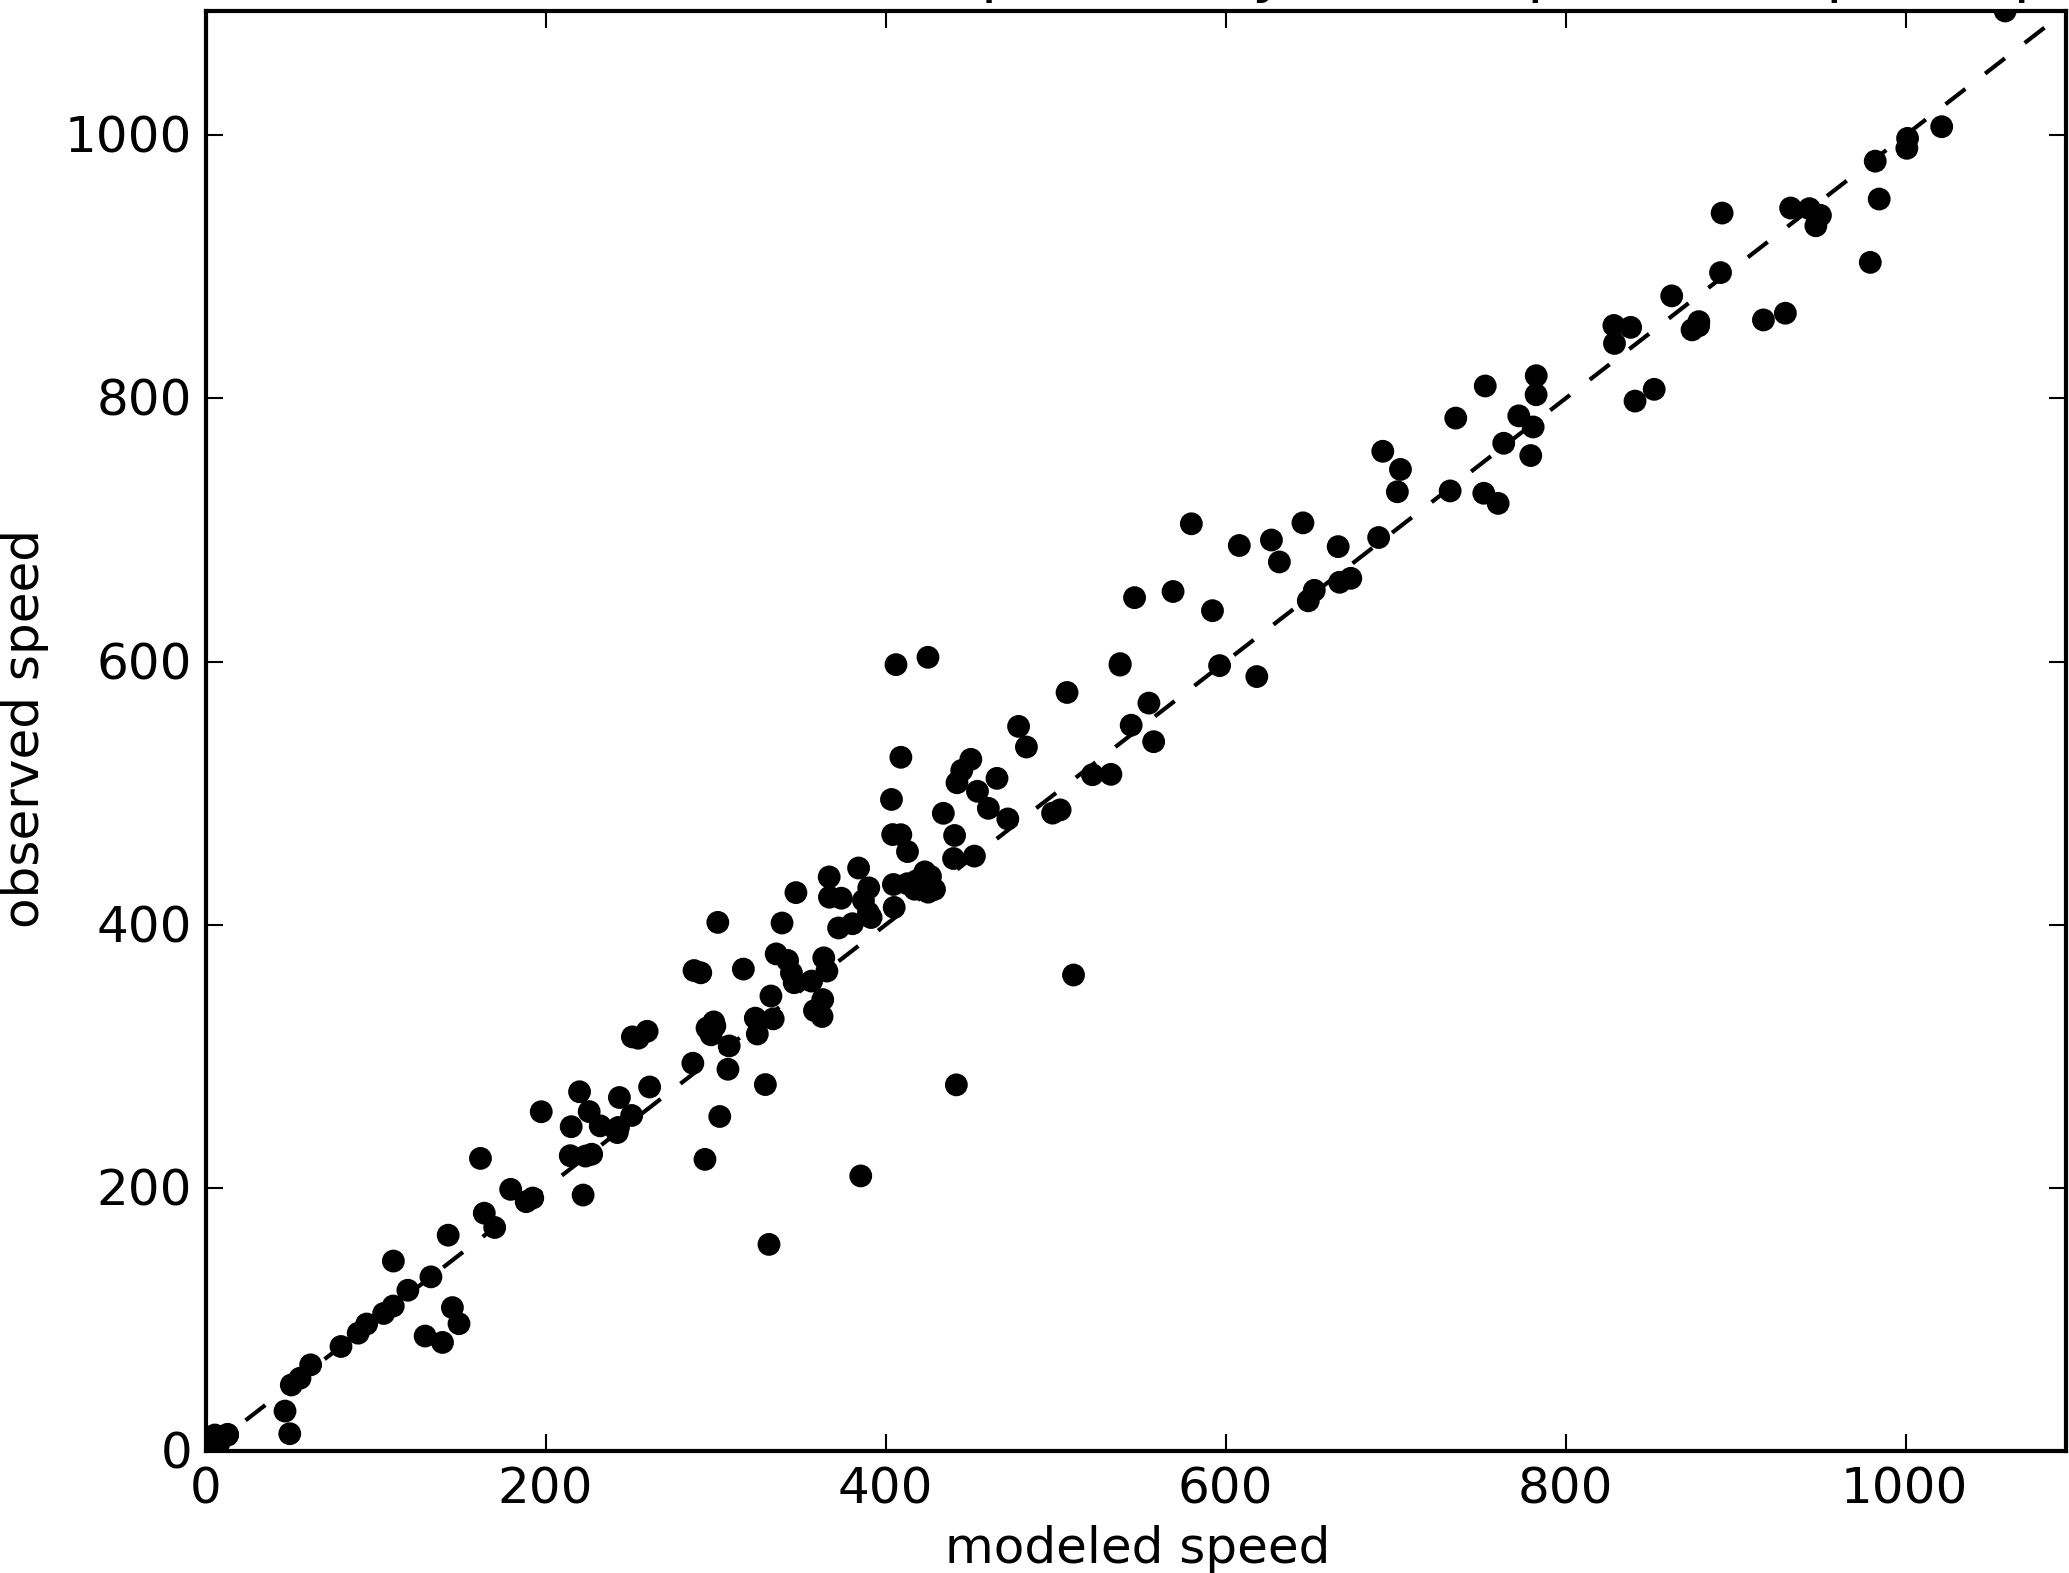
\includegraphics[width=0.45\textwidth]{rossscatter}
\end{center}
\end{frame}


\begin{frame}{numerical solution of stress balances: a summary}

\begin{itemize}
\item stress balance equations (e.g.~SSA or Stokes) determine velocity from geometry and boundary conditions
  \begin{itemize}
  \item[$\circ$] nonlinear so iteration is necessary
  \item[$\circ$] at each iteration a sparse matrix ``inner'' problem is solved \dots give it to a matrix solver software package
  \end{itemize}

\bigskip
\item general principles:
  \begin{itemize}
  \item[$\circ$] \alert{modularize your code}
  \item[$\circ$] \alert{test the parts}
  \end{itemize}
\end{itemize}
\end{frame}


\begin{frame}{the mass continuity equation: a summary}

\begin{itemize}
\item the \emph{mass continuity equation} is
  $$H_t = M - \nabla \cdot (\mathbf{u} H)$$
\item the numerical nature of this equation depends on the stress balance:
  \begin{itemize}
  \item[$\circ$] the equation is a diffusion for frozen bed, large scale flows (i.e.~SIA)
  \item[$\circ$] it is \emph{not} very diffusive for membrane stresses and no basal resistance (e.g.~SSA for ice shelves)
  \item[$\circ$] it is diffusive for ice streams (but how much?)
  \item[$\circ$] there is \emph{not} much helpful theory on this transport problem
  \item[$\circ$] \dots maybe you will help find this theory!
  \end{itemize}
\end{itemize}
\end{frame}


\begin{frame}{last idea}
\begin{itemize}
\item this thing
\begin{center}
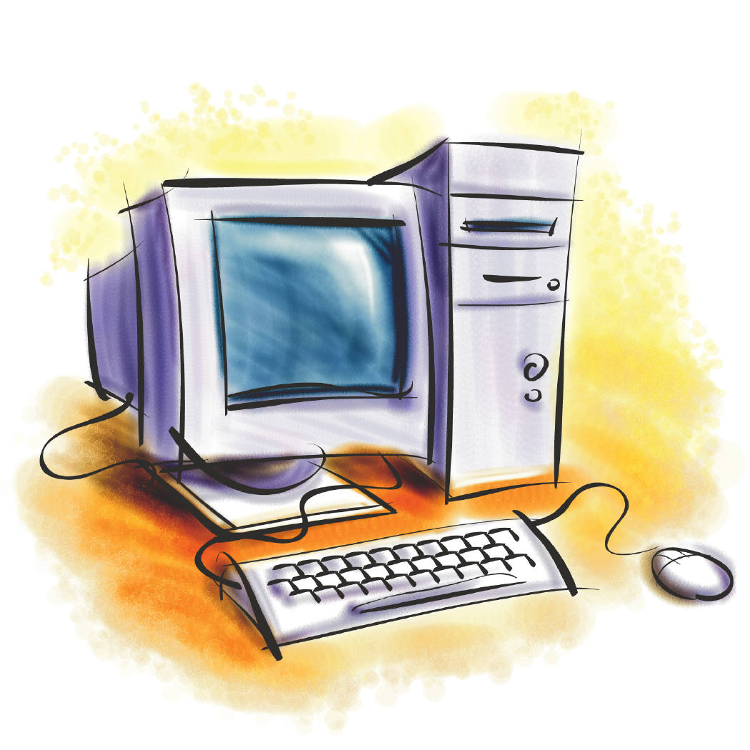
\includegraphics[width=0.3\textwidth]{computer}
\end{center}
\alert{does not know what you \emph{intend}}, but it does ``know'' your discrete model, i.e.~the program you wrote
\item \alert{all you can aspire to} is for your computer to ``know'' your continuum model, the one that you write as equations
   \begin{itemize}
   \item[$\circ$] achieve this through e.g.~verification with exact solutions
   \end{itemize}
\item but it will never hold your physical intention for the model
\end{itemize}

\end{frame}



\begin{comment}
THINK ABOUT THESE THINGS:
* SSA numerics use matrix solution: point out general sparseness and methods?  exercise related to methods?
* attempt to use Green's function to understand diffusivity of 1D SSA?
* why is ice sheet modeling a "1 bar subject"?
* make sure to test codes in Matlab
* props
   -- bicycle for plastic till analogy
   -- membrane and grid for free boundary
   -- silly putty
\end{comment}

\end{document}
